\documentclass[twoside]{book}

% Packages required by doxygen
\usepackage{fixltx2e}
\usepackage{calc}
\usepackage{doxygen}
\usepackage[export]{adjustbox} % also loads graphicx
\usepackage{graphicx}
\usepackage[utf8]{inputenc}
\usepackage{makeidx}
\usepackage{multicol}
\usepackage{multirow}
\PassOptionsToPackage{warn}{textcomp}
\usepackage{textcomp}
\usepackage[nointegrals]{wasysym}
\usepackage[table]{xcolor}

% Font selection
\usepackage[T1]{fontenc}
\usepackage[scaled=.90]{helvet}
\usepackage{courier}
\usepackage{amssymb}
\usepackage{sectsty}
\renewcommand{\familydefault}{\sfdefault}
\allsectionsfont{%
  \fontseries{bc}\selectfont%
  \color{darkgray}%
}
\renewcommand{\DoxyLabelFont}{%
  \fontseries{bc}\selectfont%
  \color{darkgray}%
}
\newcommand{\+}{\discretionary{\mbox{\scriptsize$\hookleftarrow$}}{}{}}

% Page & text layout
\usepackage{geometry}
\geometry{%
  a4paper,%
  top=2.5cm,%
  bottom=2.5cm,%
  left=2.5cm,%
  right=2.5cm%
}
\tolerance=750
\hfuzz=15pt
\hbadness=750
\setlength{\emergencystretch}{15pt}
\setlength{\parindent}{0cm}
\setlength{\parskip}{3ex plus 2ex minus 2ex}
\makeatletter
\renewcommand{\paragraph}{%
  \@startsection{paragraph}{4}{0ex}{-1.0ex}{1.0ex}{%
    \normalfont\normalsize\bfseries\SS@parafont%
  }%
}
\renewcommand{\subparagraph}{%
  \@startsection{subparagraph}{5}{0ex}{-1.0ex}{1.0ex}{%
    \normalfont\normalsize\bfseries\SS@subparafont%
  }%
}
\makeatother

% Headers & footers
\usepackage{fancyhdr}
\pagestyle{fancyplain}
\fancyhead[LE]{\fancyplain{}{\bfseries\thepage}}
\fancyhead[CE]{\fancyplain{}{}}
\fancyhead[RE]{\fancyplain{}{\bfseries\leftmark}}
\fancyhead[LO]{\fancyplain{}{\bfseries\rightmark}}
\fancyhead[CO]{\fancyplain{}{}}
\fancyhead[RO]{\fancyplain{}{\bfseries\thepage}}
\fancyfoot[LE]{\fancyplain{}{}}
\fancyfoot[CE]{\fancyplain{}{}}
\fancyfoot[RE]{\fancyplain{}{\bfseries\scriptsize Generated by Doxygen }}
\fancyfoot[LO]{\fancyplain{}{\bfseries\scriptsize Generated by Doxygen }}
\fancyfoot[CO]{\fancyplain{}{}}
\fancyfoot[RO]{\fancyplain{}{}}
\renewcommand{\footrulewidth}{0.4pt}
\renewcommand{\chaptermark}[1]{%
  \markboth{#1}{}%
}
\renewcommand{\sectionmark}[1]{%
  \markright{\thesection\ #1}%
}

% Indices & bibliography
\usepackage{natbib}
\usepackage[titles]{tocloft}
\setcounter{tocdepth}{3}
\setcounter{secnumdepth}{5}
\makeindex

% Hyperlinks (required, but should be loaded last)
\usepackage{ifpdf}
\ifpdf
  \usepackage[pdftex,pagebackref=true]{hyperref}
\else
  \usepackage[ps2pdf,pagebackref=true]{hyperref}
\fi
\hypersetup{%
  colorlinks=true,%
  linkcolor=blue,%
  citecolor=blue,%
  unicode%
}

% Custom commands
\newcommand{\clearemptydoublepage}{%
  \newpage{\pagestyle{empty}\cleardoublepage}%
}

\usepackage{caption}
\captionsetup{labelsep=space,justification=centering,font={bf},singlelinecheck=off,skip=4pt,position=top}

%===== C O N T E N T S =====

\begin{document}

% Titlepage & ToC
\hypersetup{pageanchor=false,
             bookmarksnumbered=true,
             pdfencoding=unicode
            }
\pagenumbering{alph}
\begin{titlepage}
\vspace*{7cm}
\begin{center}%
{\Large calendar }\\
\vspace*{1cm}
{\large Generated by Doxygen 1.8.13}\\
\end{center}
\end{titlepage}
\clearemptydoublepage
\pagenumbering{roman}
\tableofcontents
\clearemptydoublepage
\pagenumbering{arabic}
\hypersetup{pageanchor=true}

%--- Begin generated contents ---
\chapter{Data Structure Index}
\section{Data Structures}
Here are the data structures with brief descriptions\+:\begin{DoxyCompactList}
\item\contentsline{section}{\hyperlink{struct_event}{Event} }{\pageref{struct_event}}{}
\item\contentsline{section}{\hyperlink{struct_event_list}{Event\+List} }{\pageref{struct_event_list}}{}
\item\contentsline{section}{\hyperlink{struct_find_list}{Find\+List} }{\pageref{struct_find_list}}{}
\item\contentsline{section}{\hyperlink{struct_found_event}{Found\+Event} }{\pageref{struct_found_event}}{}
\item\contentsline{section}{\hyperlink{struct_lefoglalt}{Lefoglalt} }{\pageref{struct_lefoglalt}}{}
\item\contentsline{section}{\hyperlink{struct_menu_pont}{Menu\+Pont} }{\pageref{struct_menu_pont}}{}
\item\contentsline{section}{\hyperlink{struct_search_conditions}{Search\+Conditions} }{\pageref{struct_search_conditions}}{}
\end{DoxyCompactList}

\chapter{File Index}
\section{File List}
Here is a list of all files with brief descriptions\+:\begin{DoxyCompactList}
\item\contentsline{section}{/home/dani/\+Documents/egyetem/prog1/nagyhazi/hazi2/calendar2/calendar/\hyperlink{debugmalloc_8c}{debugmalloc.\+c} }{\pageref{debugmalloc_8c}}{}
\item\contentsline{section}{/home/dani/\+Documents/egyetem/prog1/nagyhazi/hazi2/calendar2/calendar/\hyperlink{debugmalloc_8h}{debugmalloc.\+h} }{\pageref{debugmalloc_8h}}{}
\item\contentsline{section}{/home/dani/\+Documents/egyetem/prog1/nagyhazi/hazi2/calendar2/calendar/\hyperlink{eventrecord_8c}{eventrecord.\+c} }{\pageref{eventrecord_8c}}{}
\item\contentsline{section}{/home/dani/\+Documents/egyetem/prog1/nagyhazi/hazi2/calendar2/calendar/\hyperlink{eventrecord_8h}{eventrecord.\+h} }{\pageref{eventrecord_8h}}{}
\item\contentsline{section}{/home/dani/\+Documents/egyetem/prog1/nagyhazi/hazi2/calendar2/calendar/\hyperlink{file_8c}{file.\+c} }{\pageref{file_8c}}{}
\item\contentsline{section}{/home/dani/\+Documents/egyetem/prog1/nagyhazi/hazi2/calendar2/calendar/\hyperlink{file_8h}{file.\+h} }{\pageref{file_8h}}{}
\item\contentsline{section}{/home/dani/\+Documents/egyetem/prog1/nagyhazi/hazi2/calendar2/calendar/\hyperlink{list_8c}{list.\+c} }{\pageref{list_8c}}{}
\item\contentsline{section}{/home/dani/\+Documents/egyetem/prog1/nagyhazi/hazi2/calendar2/calendar/\hyperlink{list_8h}{list.\+h} }{\pageref{list_8h}}{}
\item\contentsline{section}{/home/dani/\+Documents/egyetem/prog1/nagyhazi/hazi2/calendar2/calendar/\hyperlink{main_8c}{main.\+c} }{\pageref{main_8c}}{}
\item\contentsline{section}{/home/dani/\+Documents/egyetem/prog1/nagyhazi/hazi2/calendar2/calendar/\hyperlink{menu_8c}{menu.\+c} }{\pageref{menu_8c}}{}
\item\contentsline{section}{/home/dani/\+Documents/egyetem/prog1/nagyhazi/hazi2/calendar2/calendar/\hyperlink{menu_8h}{menu.\+h} }{\pageref{menu_8h}}{}
\item\contentsline{section}{/home/dani/\+Documents/egyetem/prog1/nagyhazi/hazi2/calendar2/calendar/\hyperlink{search_8c}{search.\+c} }{\pageref{search_8c}}{}
\item\contentsline{section}{/home/dani/\+Documents/egyetem/prog1/nagyhazi/hazi2/calendar2/calendar/\hyperlink{search_8h}{search.\+h} }{\pageref{search_8h}}{}
\item\contentsline{section}{/home/dani/\+Documents/egyetem/prog1/nagyhazi/hazi2/calendar2/calendar/\hyperlink{searchui_8c}{searchui.\+c} }{\pageref{searchui_8c}}{}
\item\contentsline{section}{/home/dani/\+Documents/egyetem/prog1/nagyhazi/hazi2/calendar2/calendar/\hyperlink{searchui_8h}{searchui.\+h} }{\pageref{searchui_8h}}{}
\item\contentsline{section}{/home/dani/\+Documents/egyetem/prog1/nagyhazi/hazi2/calendar2/calendar/\hyperlink{structures_8h}{structures.\+h} }{\pageref{structures_8h}}{}
\end{DoxyCompactList}

\chapter{Data Structure Documentation}
\hypertarget{struct_event}{}\section{Event Struct Reference}
\label{struct_event}\index{Event@{Event}}


{\ttfamily \#include $<$structures.\+h$>$}

\subsection*{Data Fields}
\begin{DoxyCompactItemize}
\item 
int \hyperlink{struct_event_abeac221e38b7b9ce7df8722c842bf671}{year}
\item 
int \hyperlink{struct_event_aedb06abe5aff12fa3e7e0e71a374edfb}{month}
\item 
int \hyperlink{struct_event_a4c11afc03fc3ee49bab660def6558f2a}{day}
\item 
int \hyperlink{struct_event_ad40616cbc61c79a6caf6c8c2464bab8d}{starthour}
\item 
int \hyperlink{struct_event_a6a7bf86ae11349bf260da9abce25452a}{startmin}
\item 
int \hyperlink{struct_event_a23ec0f5427aad3f169339f21523d2041}{endhour}
\item 
int \hyperlink{struct_event_ac9b41151b48114ff949e78b68a81572b}{endmin}
\item 
char $\ast$ \hyperlink{struct_event_a5ac083a645d964373f022d03df4849c8}{name}
\item 
char $\ast$ \hyperlink{struct_event_a6a0d5603410d5eda93c0ff341966cce1}{location}
\item 
char $\ast$ \hyperlink{struct_event_a25dae25c3bf9b28d54eb4df7afb2a491}{comment}
\item 
struct \hyperlink{struct_event}{Event} $\ast$ \hyperlink{struct_event_a306f86f79bc8a24df2ff2989f10ea5b8}{next}
\item 
struct \hyperlink{struct_event}{Event} $\ast$ \hyperlink{struct_event_a587efee11d7ca5779c56b343342c65f9}{prev}
\end{DoxyCompactItemize}


\subsection{Field Documentation}
\mbox{\Hypertarget{struct_event_a25dae25c3bf9b28d54eb4df7afb2a491}\label{struct_event_a25dae25c3bf9b28d54eb4df7afb2a491}} 
\index{Event@{Event}!comment@{comment}}
\index{comment@{comment}!Event@{Event}}
\subsubsection{\texorpdfstring{comment}{comment}}
{\footnotesize\ttfamily char$\ast$ comment}

\mbox{\Hypertarget{struct_event_a4c11afc03fc3ee49bab660def6558f2a}\label{struct_event_a4c11afc03fc3ee49bab660def6558f2a}} 
\index{Event@{Event}!day@{day}}
\index{day@{day}!Event@{Event}}
\subsubsection{\texorpdfstring{day}{day}}
{\footnotesize\ttfamily int day}

\mbox{\Hypertarget{struct_event_a23ec0f5427aad3f169339f21523d2041}\label{struct_event_a23ec0f5427aad3f169339f21523d2041}} 
\index{Event@{Event}!endhour@{endhour}}
\index{endhour@{endhour}!Event@{Event}}
\subsubsection{\texorpdfstring{endhour}{endhour}}
{\footnotesize\ttfamily int endhour}

\mbox{\Hypertarget{struct_event_ac9b41151b48114ff949e78b68a81572b}\label{struct_event_ac9b41151b48114ff949e78b68a81572b}} 
\index{Event@{Event}!endmin@{endmin}}
\index{endmin@{endmin}!Event@{Event}}
\subsubsection{\texorpdfstring{endmin}{endmin}}
{\footnotesize\ttfamily int endmin}

\mbox{\Hypertarget{struct_event_a6a0d5603410d5eda93c0ff341966cce1}\label{struct_event_a6a0d5603410d5eda93c0ff341966cce1}} 
\index{Event@{Event}!location@{location}}
\index{location@{location}!Event@{Event}}
\subsubsection{\texorpdfstring{location}{location}}
{\footnotesize\ttfamily char$\ast$ location}

\mbox{\Hypertarget{struct_event_aedb06abe5aff12fa3e7e0e71a374edfb}\label{struct_event_aedb06abe5aff12fa3e7e0e71a374edfb}} 
\index{Event@{Event}!month@{month}}
\index{month@{month}!Event@{Event}}
\subsubsection{\texorpdfstring{month}{month}}
{\footnotesize\ttfamily int month}

\mbox{\Hypertarget{struct_event_a5ac083a645d964373f022d03df4849c8}\label{struct_event_a5ac083a645d964373f022d03df4849c8}} 
\index{Event@{Event}!name@{name}}
\index{name@{name}!Event@{Event}}
\subsubsection{\texorpdfstring{name}{name}}
{\footnotesize\ttfamily char$\ast$ name}

\mbox{\Hypertarget{struct_event_a306f86f79bc8a24df2ff2989f10ea5b8}\label{struct_event_a306f86f79bc8a24df2ff2989f10ea5b8}} 
\index{Event@{Event}!next@{next}}
\index{next@{next}!Event@{Event}}
\subsubsection{\texorpdfstring{next}{next}}
{\footnotesize\ttfamily struct \hyperlink{struct_event}{Event}$\ast$ next}

\mbox{\Hypertarget{struct_event_a587efee11d7ca5779c56b343342c65f9}\label{struct_event_a587efee11d7ca5779c56b343342c65f9}} 
\index{Event@{Event}!prev@{prev}}
\index{prev@{prev}!Event@{Event}}
\subsubsection{\texorpdfstring{prev}{prev}}
{\footnotesize\ttfamily struct \hyperlink{struct_event}{Event}$\ast$ prev}

\mbox{\Hypertarget{struct_event_ad40616cbc61c79a6caf6c8c2464bab8d}\label{struct_event_ad40616cbc61c79a6caf6c8c2464bab8d}} 
\index{Event@{Event}!starthour@{starthour}}
\index{starthour@{starthour}!Event@{Event}}
\subsubsection{\texorpdfstring{starthour}{starthour}}
{\footnotesize\ttfamily int starthour}

\mbox{\Hypertarget{struct_event_a6a7bf86ae11349bf260da9abce25452a}\label{struct_event_a6a7bf86ae11349bf260da9abce25452a}} 
\index{Event@{Event}!startmin@{startmin}}
\index{startmin@{startmin}!Event@{Event}}
\subsubsection{\texorpdfstring{startmin}{startmin}}
{\footnotesize\ttfamily int startmin}

\mbox{\Hypertarget{struct_event_abeac221e38b7b9ce7df8722c842bf671}\label{struct_event_abeac221e38b7b9ce7df8722c842bf671}} 
\index{Event@{Event}!year@{year}}
\index{year@{year}!Event@{Event}}
\subsubsection{\texorpdfstring{year}{year}}
{\footnotesize\ttfamily int year}



The documentation for this struct was generated from the following file\+:\begin{DoxyCompactItemize}
\item 
/home/dani/\+Documents/egyetem/prog1/nagyhazi/hazi2/calendar2/calendar/\hyperlink{structures_8h}{structures.\+h}\end{DoxyCompactItemize}

\hypertarget{struct_event_list}{}\section{Event\+List Struct Reference}
\label{struct_event_list}\index{Event\+List@{Event\+List}}


{\ttfamily \#include $<$structures.\+h$>$}



Collaboration diagram for Event\+List\+:\nopagebreak
\begin{figure}[H]
\begin{center}
\leavevmode
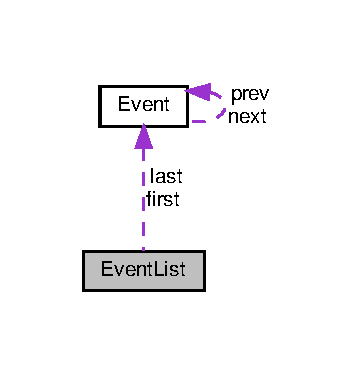
\includegraphics[width=170pt]{struct_event_list__coll__graph}
\end{center}
\end{figure}
\subsection*{Data Fields}
\begin{DoxyCompactItemize}
\item 
\hyperlink{struct_event}{Event} $\ast$ \hyperlink{struct_event_list_ab866d72c6e161e5eb85d4940b0dbc62e}{first}
\item 
\hyperlink{struct_event}{Event} $\ast$ \hyperlink{struct_event_list_a8e52f53a3606d45d86182ce606e9369d}{last}
\end{DoxyCompactItemize}


\subsection{Field Documentation}
\mbox{\Hypertarget{struct_event_list_ab866d72c6e161e5eb85d4940b0dbc62e}\label{struct_event_list_ab866d72c6e161e5eb85d4940b0dbc62e}} 
\index{Event\+List@{Event\+List}!first@{first}}
\index{first@{first}!Event\+List@{Event\+List}}
\subsubsection{\texorpdfstring{first}{first}}
{\footnotesize\ttfamily \hyperlink{struct_event}{Event}$\ast$ first}

\mbox{\Hypertarget{struct_event_list_a8e52f53a3606d45d86182ce606e9369d}\label{struct_event_list_a8e52f53a3606d45d86182ce606e9369d}} 
\index{Event\+List@{Event\+List}!last@{last}}
\index{last@{last}!Event\+List@{Event\+List}}
\subsubsection{\texorpdfstring{last}{last}}
{\footnotesize\ttfamily \hyperlink{struct_event}{Event}$\ast$ last}



The documentation for this struct was generated from the following file\+:\begin{DoxyCompactItemize}
\item 
/home/dani/\+Documents/egyetem/prog1/nagyhazi/hazi2/calendar2/calendar/\hyperlink{structures_8h}{structures.\+h}\end{DoxyCompactItemize}

\hypertarget{struct_find_list}{}\section{Find\+List Struct Reference}
\label{struct_find_list}\index{Find\+List@{Find\+List}}


{\ttfamily \#include $<$structures.\+h$>$}

\subsection*{Data Fields}
\begin{DoxyCompactItemize}
\item 
\hyperlink{struct_found_event}{Found\+Event} $\ast$ \hyperlink{struct_find_list_a9f9781ae49412999177095cb5e8c79d1}{first}
\item 
\hyperlink{struct_found_event}{Found\+Event} $\ast$ \hyperlink{struct_find_list_ab61e64643b8233c6d9feef3e2aaffef2}{last}
\end{DoxyCompactItemize}


\subsection{Detailed Description}
A keresés által talált események listája 

\subsection{Field Documentation}
\mbox{\Hypertarget{struct_find_list_a9f9781ae49412999177095cb5e8c79d1}\label{struct_find_list_a9f9781ae49412999177095cb5e8c79d1}} 
\index{Find\+List@{Find\+List}!first@{first}}
\index{first@{first}!Find\+List@{Find\+List}}
\subsubsection{\texorpdfstring{first}{first}}
{\footnotesize\ttfamily \hyperlink{struct_found_event}{Found\+Event}$\ast$ first}

a találati lista első őrszeme, üres \mbox{\Hypertarget{struct_find_list_ab61e64643b8233c6d9feef3e2aaffef2}\label{struct_find_list_ab61e64643b8233c6d9feef3e2aaffef2}} 
\index{Find\+List@{Find\+List}!last@{last}}
\index{last@{last}!Find\+List@{Find\+List}}
\subsubsection{\texorpdfstring{last}{last}}
{\footnotesize\ttfamily \hyperlink{struct_found_event}{Found\+Event}$\ast$ last}

a találati lista utolsó őrszeme, üres 

The documentation for this struct was generated from the following file\+:\begin{DoxyCompactItemize}
\item 
/home/dani/\+Documents/egyetem/prog1/nagyhazi/hazi2/calendar2/calendar/\hyperlink{structures_8h}{structures.\+h}\end{DoxyCompactItemize}

\hypertarget{struct_found_event}{}\section{Found\+Event Struct Reference}
\label{struct_found_event}\index{Found\+Event@{Found\+Event}}


{\ttfamily \#include $<$structures.\+h$>$}

\subsection*{Data Fields}
\begin{DoxyCompactItemize}
\item 
\hyperlink{struct_event}{Event} $\ast$ \hyperlink{struct_found_event_a9fb10dd8687d775ac50c8824bde19d67}{foundevent}
\item 
struct \hyperlink{struct_found_event}{Found\+Event} $\ast$ \hyperlink{struct_found_event_add29159b298db5eb8c68bd9314e7c498}{prevfound}
\item 
struct \hyperlink{struct_found_event}{Found\+Event} $\ast$ \hyperlink{struct_found_event_acbce65ffd090e8c5d45aa15b2ccdf453}{nextfound}
\end{DoxyCompactItemize}


\subsection{Field Documentation}
\mbox{\Hypertarget{struct_found_event_a9fb10dd8687d775ac50c8824bde19d67}\label{struct_found_event_a9fb10dd8687d775ac50c8824bde19d67}} 
\index{Found\+Event@{Found\+Event}!foundevent@{foundevent}}
\index{foundevent@{foundevent}!Found\+Event@{Found\+Event}}
\subsubsection{\texorpdfstring{foundevent}{foundevent}}
{\footnotesize\ttfamily \hyperlink{struct_event}{Event}$\ast$ foundevent}

\mbox{\Hypertarget{struct_found_event_acbce65ffd090e8c5d45aa15b2ccdf453}\label{struct_found_event_acbce65ffd090e8c5d45aa15b2ccdf453}} 
\index{Found\+Event@{Found\+Event}!nextfound@{nextfound}}
\index{nextfound@{nextfound}!Found\+Event@{Found\+Event}}
\subsubsection{\texorpdfstring{nextfound}{nextfound}}
{\footnotesize\ttfamily struct \hyperlink{struct_found_event}{Found\+Event}$\ast$ nextfound}

\mbox{\Hypertarget{struct_found_event_add29159b298db5eb8c68bd9314e7c498}\label{struct_found_event_add29159b298db5eb8c68bd9314e7c498}} 
\index{Found\+Event@{Found\+Event}!prevfound@{prevfound}}
\index{prevfound@{prevfound}!Found\+Event@{Found\+Event}}
\subsubsection{\texorpdfstring{prevfound}{prevfound}}
{\footnotesize\ttfamily struct \hyperlink{struct_found_event}{Found\+Event}$\ast$ prevfound}



The documentation for this struct was generated from the following file\+:\begin{DoxyCompactItemize}
\item 
/home/dani/\+Documents/egyetem/prog1/nagyhazi/hazi2/calendar2/calendar/\hyperlink{structures_8h}{structures.\+h}\end{DoxyCompactItemize}

\hypertarget{struct_menu_pont}{}\section{Menu\+Pont Struct Reference}
\label{struct_menu_pont}\index{Menu\+Pont@{Menu\+Pont}}


{\ttfamily \#include $<$structures.\+h$>$}

\subsection*{Data Fields}
\begin{DoxyCompactItemize}
\item 
char const  $\ast$ \hyperlink{struct_menu_pont_a21c8b004e3b92cd18b29f8a51717956d}{nev}
\end{DoxyCompactItemize}


\subsection{Detailed Description}
Menupontok neveinek listája 

\subsection{Field Documentation}
\mbox{\Hypertarget{struct_menu_pont_a21c8b004e3b92cd18b29f8a51717956d}\label{struct_menu_pont_a21c8b004e3b92cd18b29f8a51717956d}} 
\index{Menu\+Pont@{Menu\+Pont}!nev@{nev}}
\index{nev@{nev}!Menu\+Pont@{Menu\+Pont}}
\subsubsection{\texorpdfstring{nev}{nev}}
{\footnotesize\ttfamily char const$\ast$ nev}

menüpont nevére mutató karaktertömb 

The documentation for this struct was generated from the following file\+:\begin{DoxyCompactItemize}
\item 
/home/dani/\+Documents/egyetem/prog1/nagyhazi/hazi2/calendar2/calendar/\hyperlink{structures_8h}{structures.\+h}\end{DoxyCompactItemize}

\hypertarget{struct_search_conditions}{}\section{Search\+Conditions Struct Reference}
\label{struct_search_conditions}\index{Search\+Conditions@{Search\+Conditions}}


{\ttfamily \#include $<$structures.\+h$>$}

\subsection*{Data Fields}
\begin{DoxyCompactItemize}
\item 
char $\ast$ \hyperlink{struct_search_conditions_a5ac083a645d964373f022d03df4849c8}{name}
\item 
int \hyperlink{struct_search_conditions_abeac221e38b7b9ce7df8722c842bf671}{year}
\item 
int \hyperlink{struct_search_conditions_a3560bdec25d509ef8f4f02409eaa9f1d}{week}
\item 
int \hyperlink{struct_search_conditions_aedb06abe5aff12fa3e7e0e71a374edfb}{month}
\item 
int \hyperlink{struct_search_conditions_a4c11afc03fc3ee49bab660def6558f2a}{day}
\end{DoxyCompactItemize}


\subsection{Field Documentation}
\mbox{\Hypertarget{struct_search_conditions_a4c11afc03fc3ee49bab660def6558f2a}\label{struct_search_conditions_a4c11afc03fc3ee49bab660def6558f2a}} 
\index{Search\+Conditions@{Search\+Conditions}!day@{day}}
\index{day@{day}!Search\+Conditions@{Search\+Conditions}}
\subsubsection{\texorpdfstring{day}{day}}
{\footnotesize\ttfamily int day}

\mbox{\Hypertarget{struct_search_conditions_aedb06abe5aff12fa3e7e0e71a374edfb}\label{struct_search_conditions_aedb06abe5aff12fa3e7e0e71a374edfb}} 
\index{Search\+Conditions@{Search\+Conditions}!month@{month}}
\index{month@{month}!Search\+Conditions@{Search\+Conditions}}
\subsubsection{\texorpdfstring{month}{month}}
{\footnotesize\ttfamily int month}

\mbox{\Hypertarget{struct_search_conditions_a5ac083a645d964373f022d03df4849c8}\label{struct_search_conditions_a5ac083a645d964373f022d03df4849c8}} 
\index{Search\+Conditions@{Search\+Conditions}!name@{name}}
\index{name@{name}!Search\+Conditions@{Search\+Conditions}}
\subsubsection{\texorpdfstring{name}{name}}
{\footnotesize\ttfamily char$\ast$ name}

\mbox{\Hypertarget{struct_search_conditions_a3560bdec25d509ef8f4f02409eaa9f1d}\label{struct_search_conditions_a3560bdec25d509ef8f4f02409eaa9f1d}} 
\index{Search\+Conditions@{Search\+Conditions}!week@{week}}
\index{week@{week}!Search\+Conditions@{Search\+Conditions}}
\subsubsection{\texorpdfstring{week}{week}}
{\footnotesize\ttfamily int week}

\mbox{\Hypertarget{struct_search_conditions_abeac221e38b7b9ce7df8722c842bf671}\label{struct_search_conditions_abeac221e38b7b9ce7df8722c842bf671}} 
\index{Search\+Conditions@{Search\+Conditions}!year@{year}}
\index{year@{year}!Search\+Conditions@{Search\+Conditions}}
\subsubsection{\texorpdfstring{year}{year}}
{\footnotesize\ttfamily int year}



The documentation for this struct was generated from the following file\+:\begin{DoxyCompactItemize}
\item 
/home/dani/\+Documents/egyetem/prog1/nagyhazi/hazi2/calendar2/calendar/\hyperlink{structures_8h}{structures.\+h}\end{DoxyCompactItemize}

\chapter{File Documentation}
\hypertarget{eventrecord_8c}{}\section{/home/dani/\+Documents/egyetem/prog1/nagyhazi/hazi2/calendar2/calendar/eventrecord.c File Reference}
\label{eventrecord_8c}\index{/home/dani/\+Documents/egyetem/prog1/nagyhazi/hazi2/calendar2/calendar/eventrecord.\+c@{/home/dani/\+Documents/egyetem/prog1/nagyhazi/hazi2/calendar2/calendar/eventrecord.\+c}}
{\ttfamily \#include \char`\"{}eventrecord.\+h\char`\"{}}\newline
{\ttfamily \#include \char`\"{}structures.\+h\char`\"{}}\newline
{\ttfamily \#include $<$stdio.\+h$>$}\newline
{\ttfamily \#include $<$stdbool.\+h$>$}\newline
{\ttfamily \#include \char`\"{}menu.\+h\char`\"{}}\newline
{\ttfamily \#include \char`\"{}list.\+h\char`\"{}}\newline
{\ttfamily \#include $<$stdlib.\+h$>$}\newline
\subsection*{Functions}
\begin{DoxyCompactItemize}
\item 
void \hyperlink{group__eventrecord_ga610dc34a1e251a16311ca7ac15f64e05}{moveevent} (\hyperlink{struct_event}{Event} $\ast$event, \hyperlink{struct_event_list}{Event\+List} const $\ast$eventlist, \hyperlink{group__eventrecord_ga643f8b09cbc45afc4ad36b27c077b1fd}{Mod\+By} modby)
\item 
void \hyperlink{group__eventrecord_gaf69a5ee77b139263897d5e6bfe7d7f2a}{deleteevent} (\hyperlink{struct_event}{Event} $\ast$event)
\item 
int \hyperlink{group__eventrecord_gac6e06e3186496cd8eb6618baf3ca9d3e}{scanrecordcommand} (bool isnewevent, int i, \hyperlink{struct_event}{Event} $\ast$event, \hyperlink{struct_event_list}{Event\+List} const $\ast$eventlist)
\item 
int \hyperlink{group__eventrecord_ga43a7dc247171d596d8d808776d8d40f5}{printeventrecord} (\hyperlink{struct_event}{Event} $\ast$event, \hyperlink{struct_search_conditions}{Search\+Conditions} condition, \hyperlink{struct_event_list}{Event\+List} $\ast$eventlist)
\end{DoxyCompactItemize}

\hypertarget{eventrecord_8h}{}\section{/home/dani/\+Documents/egyetem/prog1/nagyhazi/hazi2/calendar2/calendar/eventrecord.h File Reference}
\label{eventrecord_8h}\index{/home/dani/\+Documents/egyetem/prog1/nagyhazi/hazi2/calendar2/calendar/eventrecord.\+h@{/home/dani/\+Documents/egyetem/prog1/nagyhazi/hazi2/calendar2/calendar/eventrecord.\+h}}
{\ttfamily \#include \char`\"{}structures.\+h\char`\"{}}\newline
Include dependency graph for eventrecord.\+h\+:\nopagebreak
\begin{figure}[H]
\begin{center}
\leavevmode
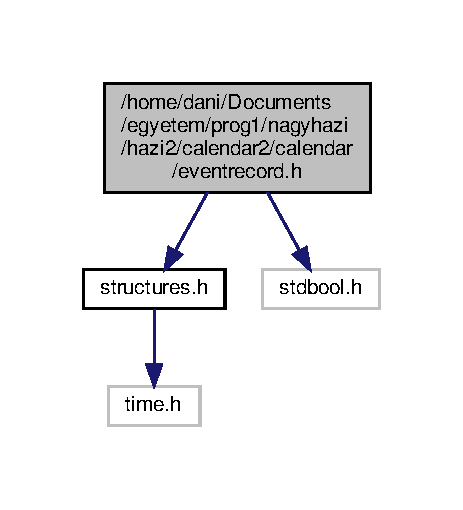
\includegraphics[width=208pt]{eventrecord_8h__incl}
\end{center}
\end{figure}
This graph shows which files directly or indirectly include this file\+:
\nopagebreak
\begin{figure}[H]
\begin{center}
\leavevmode
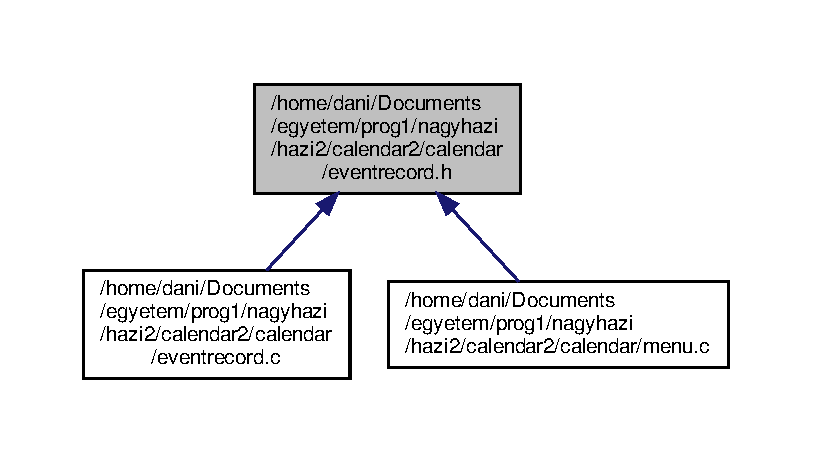
\includegraphics[width=350pt]{eventrecord_8h__dep__incl}
\end{center}
\end{figure}

\hypertarget{file_8c}{}\section{/home/dani/\+Documents/egyetem/prog1/nagyhazi/hazi2/calendar2/calendar/file.c File Reference}
\label{file_8c}\index{/home/dani/\+Documents/egyetem/prog1/nagyhazi/hazi2/calendar2/calendar/file.\+c@{/home/dani/\+Documents/egyetem/prog1/nagyhazi/hazi2/calendar2/calendar/file.\+c}}
{\ttfamily \#include \char`\"{}file.\+h\char`\"{}}\newline
{\ttfamily \#include $<$stdio.\+h$>$}\newline
{\ttfamily \#include $<$stdbool.\+h$>$}\newline
{\ttfamily \#include \char`\"{}structures.\+h\char`\"{}}\newline
{\ttfamily \#include \char`\"{}list.\+h\char`\"{}}\newline
{\ttfamily \#include $<$string.\+h$>$}\newline
{\ttfamily \#include $<$stdlib.\+h$>$}\newline
\subsection*{Functions}
\begin{DoxyCompactItemize}
\item 
char $\ast$ \hyperlink{group__file_ga91b52505951ff88321e947b6e1c4b779}{dstrcpy} (char const $\ast$str)
\item 
bool \hyperlink{group__file_gaf4efa1e078c7552b2f70daf3a40039c7}{calendarload} (\hyperlink{struct_event_list}{Event\+List} const $\ast$eventlist)
\item 
bool \hyperlink{group__file_ga7f69872489b7c1c4bcdd125319a87b2e}{calendarsave} (\hyperlink{struct_event_list}{Event\+List} const $\ast$eventlist)
\end{DoxyCompactItemize}

\hypertarget{file_8h}{}\section{/home/dani/\+Documents/egyetem/prog1/nagyhazi/hazi2/calendar2/calendar/file.h File Reference}
\label{file_8h}\index{/home/dani/\+Documents/egyetem/prog1/nagyhazi/hazi2/calendar2/calendar/file.\+h@{/home/dani/\+Documents/egyetem/prog1/nagyhazi/hazi2/calendar2/calendar/file.\+h}}
{\ttfamily \#include $<$stdio.\+h$>$}\newline
{\ttfamily \#include \char`\"{}structures.\+h\char`\"{}}\newline
Include dependency graph for file.\+h\+:\nopagebreak
\begin{figure}[H]
\begin{center}
\leavevmode
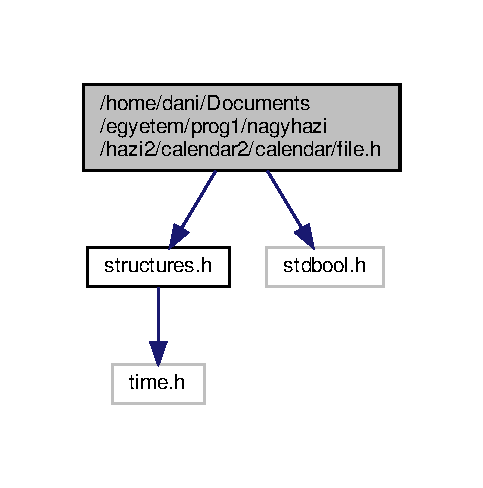
\includegraphics[width=232pt]{file_8h__incl}
\end{center}
\end{figure}
This graph shows which files directly or indirectly include this file\+:\nopagebreak
\begin{figure}[H]
\begin{center}
\leavevmode
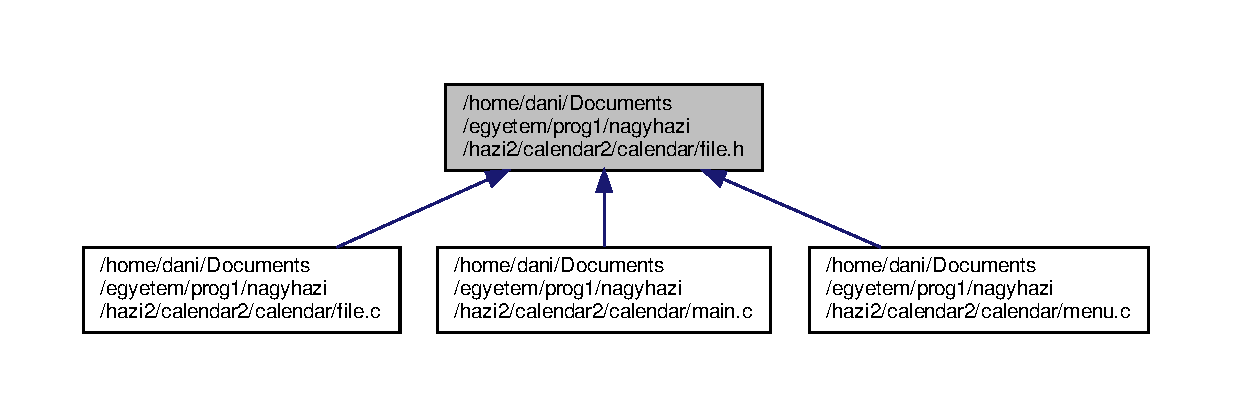
\includegraphics[width=350pt]{file_8h__dep__incl}
\end{center}
\end{figure}
\subsection*{Functions}
\begin{DoxyCompactItemize}
\item 
void \hyperlink{file_8h_a31d677237f8b1f618a6183133eae616d}{fileload} ()
\item 
void \hyperlink{file_8h_afc715bc6c0b9a9e85af15dc509a8d34b}{filesave} (\hyperlink{struct_event_list}{Event\+List} $\ast$eventlist)
\end{DoxyCompactItemize}


\subsection{Function Documentation}
\mbox{\Hypertarget{file_8h_a31d677237f8b1f618a6183133eae616d}\label{file_8h_a31d677237f8b1f618a6183133eae616d}} 
\index{file.\+h@{file.\+h}!fileload@{fileload}}
\index{fileload@{fileload}!file.\+h@{file.\+h}}
\subsubsection{\texorpdfstring{fileload()}{fileload()}}
{\footnotesize\ttfamily void fileload (\begin{DoxyParamCaption}{ }\end{DoxyParamCaption})}

\mbox{\Hypertarget{file_8h_afc715bc6c0b9a9e85af15dc509a8d34b}\label{file_8h_afc715bc6c0b9a9e85af15dc509a8d34b}} 
\index{file.\+h@{file.\+h}!filesave@{filesave}}
\index{filesave@{filesave}!file.\+h@{file.\+h}}
\subsubsection{\texorpdfstring{filesave()}{filesave()}}
{\footnotesize\ttfamily void filesave (\begin{DoxyParamCaption}\item[{\hyperlink{struct_event_list}{Event\+List} $\ast$}]{eventlist }\end{DoxyParamCaption})}

Here is the call graph for this function\+:
\nopagebreak
\begin{figure}[H]
\begin{center}
\leavevmode
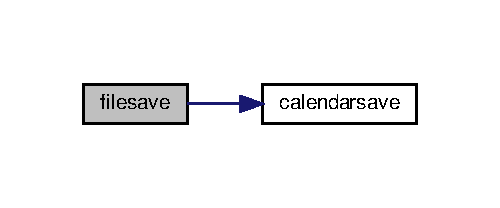
\includegraphics[width=240pt]{file_8h_afc715bc6c0b9a9e85af15dc509a8d34b_cgraph}
\end{center}
\end{figure}
Here is the caller graph for this function\+:
\nopagebreak
\begin{figure}[H]
\begin{center}
\leavevmode
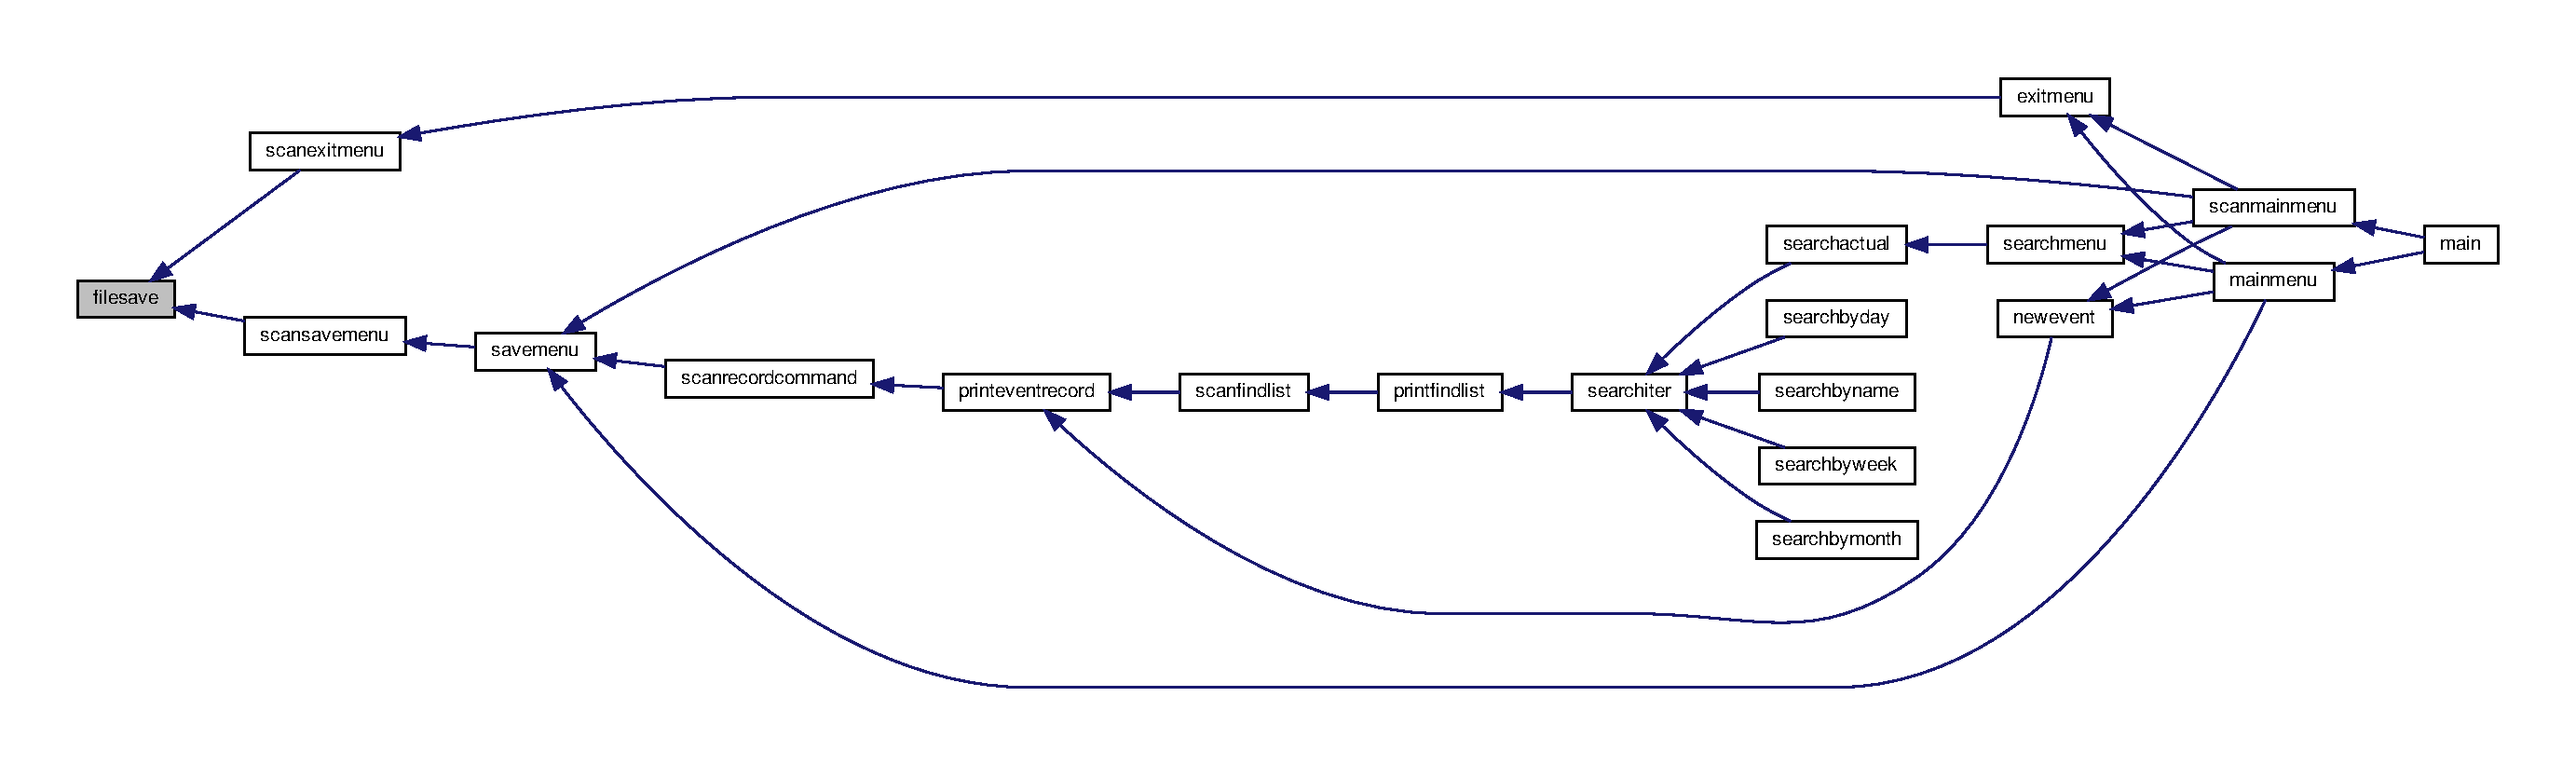
\includegraphics[width=350pt]{file_8h_afc715bc6c0b9a9e85af15dc509a8d34b_icgraph}
\end{center}
\end{figure}

\hypertarget{list_8c}{}\section{/home/dani/\+Documents/egyetem/prog1/nagyhazi/hazi2/calendar2/calendar/list.c File Reference}
\label{list_8c}\index{/home/dani/\+Documents/egyetem/prog1/nagyhazi/hazi2/calendar2/calendar/list.\+c@{/home/dani/\+Documents/egyetem/prog1/nagyhazi/hazi2/calendar2/calendar/list.\+c}}
{\ttfamily \#include \char`\"{}list.\+h\char`\"{}}\newline
{\ttfamily \#include $<$stdlib.\+h$>$}\newline
{\ttfamily \#include \char`\"{}structures.\+h\char`\"{}}\newline
{\ttfamily \#include $<$time.\+h$>$}\newline
Include dependency graph for list.\+c\+:\nopagebreak
\begin{figure}[H]
\begin{center}
\leavevmode
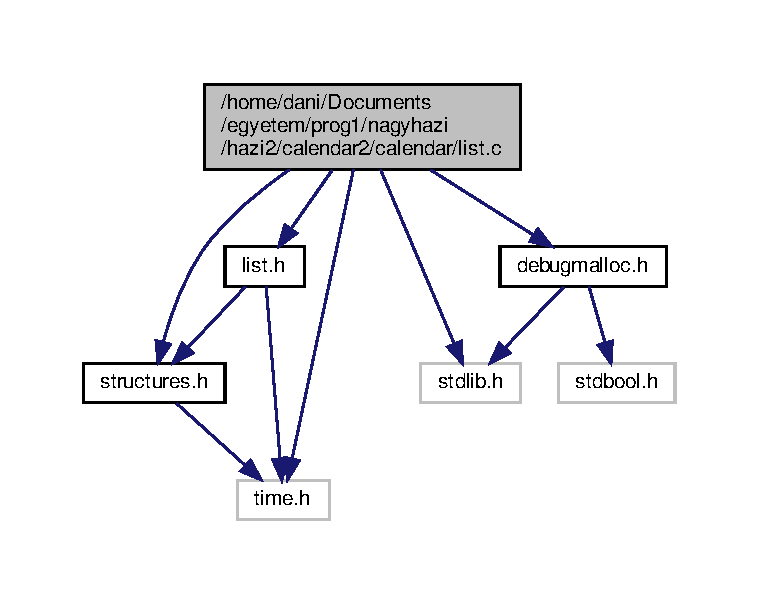
\includegraphics[width=290pt]{list_8c__incl}
\end{center}
\end{figure}
\subsection*{Functions}
\begin{DoxyCompactItemize}
\item 
\hyperlink{struct_event_list}{Event\+List} $\ast$ \hyperlink{list_8c_a48f44148563512bd32274821f478bd1b}{initeventlist} ()
\item 
\hyperlink{struct_event}{Event} $\ast$ \hyperlink{list_8c_a24fd1b37eee54600b66c42e86b52244a}{createevent} (int ev, int honap, int nap, int ora, int perc, int bora, int bperc, char $\ast$nev, char $\ast$hely, char $\ast$comment)
\item 
void \hyperlink{list_8c_a7ef519287e473ee333204280a5d91403}{insertevent} (\hyperlink{struct_event_list}{Event\+List} $\ast$eventlist, \hyperlink{struct_event}{Event} $\ast$event)
\item 
int \hyperlink{list_8c_a8f7708495c6e39bb6e712218711b331f}{starttime} (\hyperlink{struct_event}{Event} $\ast$event)
\item 
void \hyperlink{list_8c_a2561d96be1299fd3f5730c6d82143709}{printevent\+\_\+short} (\hyperlink{struct_event}{Event} $\ast$event)
\end{DoxyCompactItemize}


\subsection{Function Documentation}
\mbox{\Hypertarget{list_8c_a24fd1b37eee54600b66c42e86b52244a}\label{list_8c_a24fd1b37eee54600b66c42e86b52244a}} 
\index{list.\+c@{list.\+c}!createevent@{createevent}}
\index{createevent@{createevent}!list.\+c@{list.\+c}}
\subsubsection{\texorpdfstring{createevent()}{createevent()}}
{\footnotesize\ttfamily \hyperlink{struct_event}{Event}$\ast$ createevent (\begin{DoxyParamCaption}\item[{int}]{ev,  }\item[{int}]{honap,  }\item[{int}]{nap,  }\item[{int}]{ora,  }\item[{int}]{perc,  }\item[{int}]{bora,  }\item[{int}]{bperc,  }\item[{char $\ast$}]{nev,  }\item[{char $\ast$}]{hely,  }\item[{char $\ast$}]{comment }\end{DoxyParamCaption})}

Here is the caller graph for this function\+:
\nopagebreak
\begin{figure}[H]
\begin{center}
\leavevmode
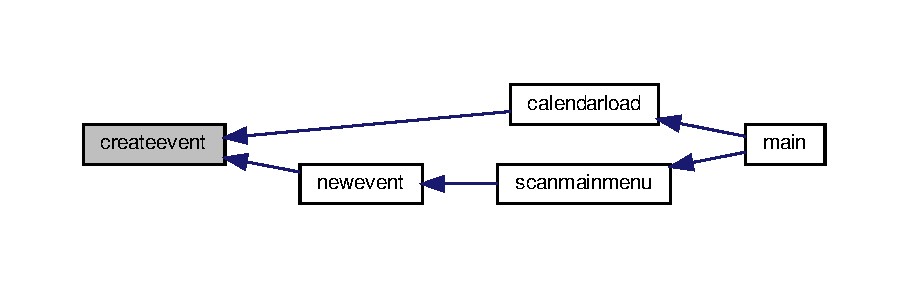
\includegraphics[width=350pt]{list_8c_a24fd1b37eee54600b66c42e86b52244a_icgraph}
\end{center}
\end{figure}
\mbox{\Hypertarget{list_8c_a48f44148563512bd32274821f478bd1b}\label{list_8c_a48f44148563512bd32274821f478bd1b}} 
\index{list.\+c@{list.\+c}!initeventlist@{initeventlist}}
\index{initeventlist@{initeventlist}!list.\+c@{list.\+c}}
\subsubsection{\texorpdfstring{initeventlist()}{initeventlist()}}
{\footnotesize\ttfamily \hyperlink{struct_event_list}{Event\+List}$\ast$ initeventlist (\begin{DoxyParamCaption}{ }\end{DoxyParamCaption})}

Here is the caller graph for this function\+:
\nopagebreak
\begin{figure}[H]
\begin{center}
\leavevmode
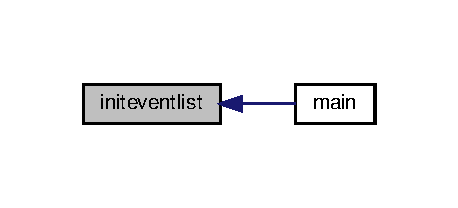
\includegraphics[width=220pt]{list_8c_a48f44148563512bd32274821f478bd1b_icgraph}
\end{center}
\end{figure}
\mbox{\Hypertarget{list_8c_a7ef519287e473ee333204280a5d91403}\label{list_8c_a7ef519287e473ee333204280a5d91403}} 
\index{list.\+c@{list.\+c}!insertevent@{insertevent}}
\index{insertevent@{insertevent}!list.\+c@{list.\+c}}
\subsubsection{\texorpdfstring{insertevent()}{insertevent()}}
{\footnotesize\ttfamily void insertevent (\begin{DoxyParamCaption}\item[{\hyperlink{struct_event_list}{Event\+List} $\ast$}]{eventlist,  }\item[{\hyperlink{struct_event}{Event} $\ast$}]{event }\end{DoxyParamCaption})}

Here is the call graph for this function\+:
\nopagebreak
\begin{figure}[H]
\begin{center}
\leavevmode
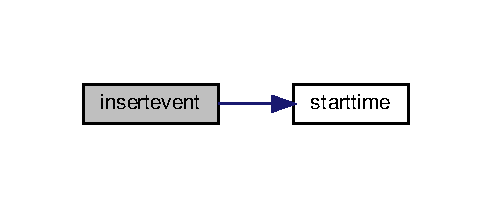
\includegraphics[width=236pt]{list_8c_a7ef519287e473ee333204280a5d91403_cgraph}
\end{center}
\end{figure}
Here is the caller graph for this function\+:
\nopagebreak
\begin{figure}[H]
\begin{center}
\leavevmode
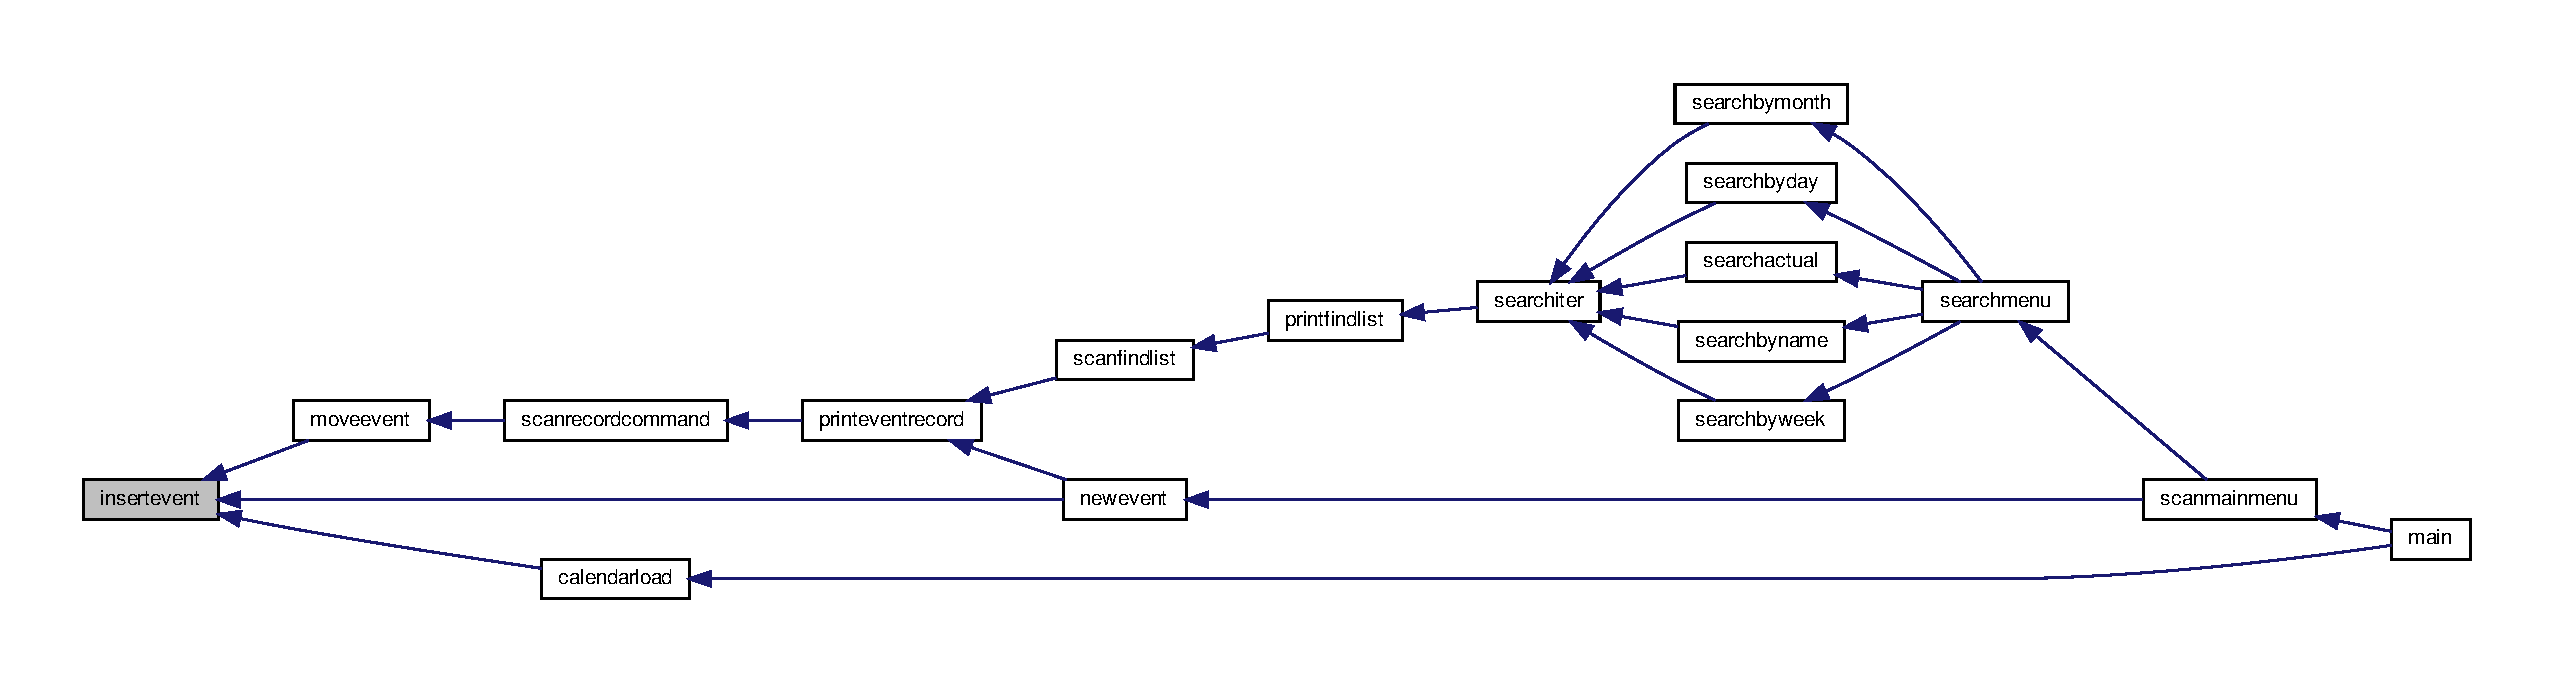
\includegraphics[width=350pt]{list_8c_a7ef519287e473ee333204280a5d91403_icgraph}
\end{center}
\end{figure}
\mbox{\Hypertarget{list_8c_a2561d96be1299fd3f5730c6d82143709}\label{list_8c_a2561d96be1299fd3f5730c6d82143709}} 
\index{list.\+c@{list.\+c}!printevent\+\_\+short@{printevent\+\_\+short}}
\index{printevent\+\_\+short@{printevent\+\_\+short}!list.\+c@{list.\+c}}
\subsubsection{\texorpdfstring{printevent\+\_\+short()}{printevent\_short()}}
{\footnotesize\ttfamily void printevent\+\_\+short (\begin{DoxyParamCaption}\item[{\hyperlink{struct_event}{Event} $\ast$}]{event }\end{DoxyParamCaption})}

Here is the caller graph for this function\+:
\nopagebreak
\begin{figure}[H]
\begin{center}
\leavevmode
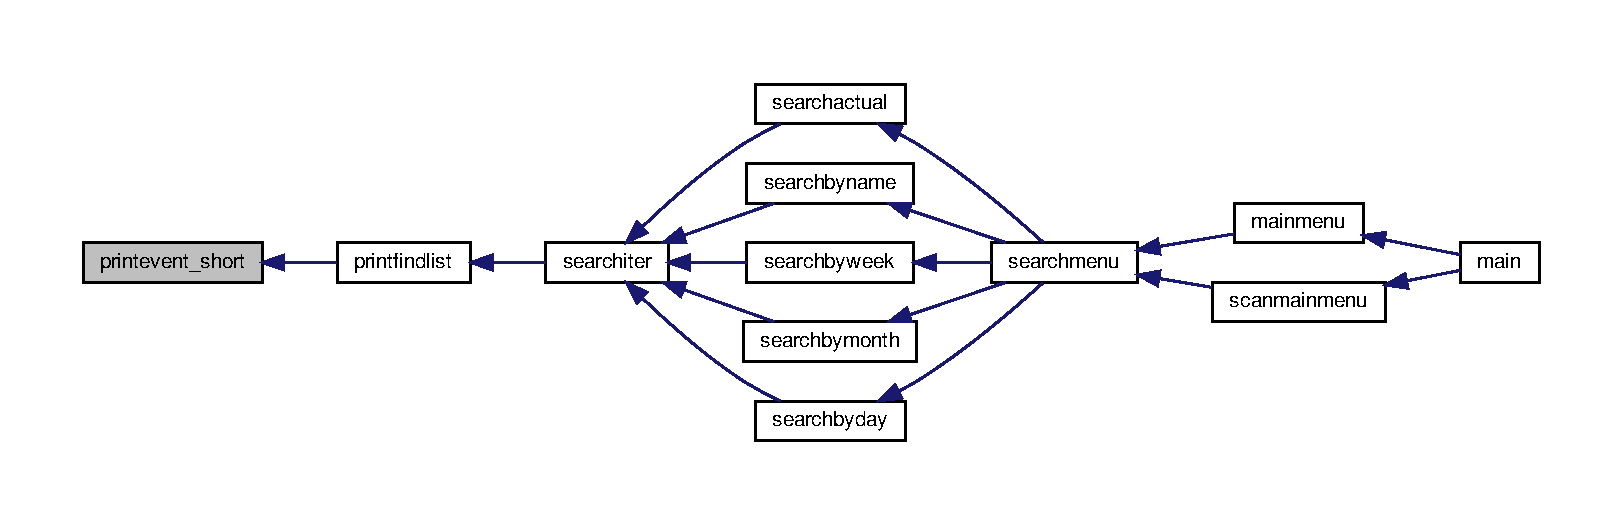
\includegraphics[width=350pt]{list_8c_a2561d96be1299fd3f5730c6d82143709_icgraph}
\end{center}
\end{figure}
\mbox{\Hypertarget{list_8c_a8f7708495c6e39bb6e712218711b331f}\label{list_8c_a8f7708495c6e39bb6e712218711b331f}} 
\index{list.\+c@{list.\+c}!starttime@{starttime}}
\index{starttime@{starttime}!list.\+c@{list.\+c}}
\subsubsection{\texorpdfstring{starttime()}{starttime()}}
{\footnotesize\ttfamily int starttime (\begin{DoxyParamCaption}\item[{\hyperlink{struct_event}{Event} $\ast$}]{event }\end{DoxyParamCaption})}

Here is the caller graph for this function\+:
\nopagebreak
\begin{figure}[H]
\begin{center}
\leavevmode
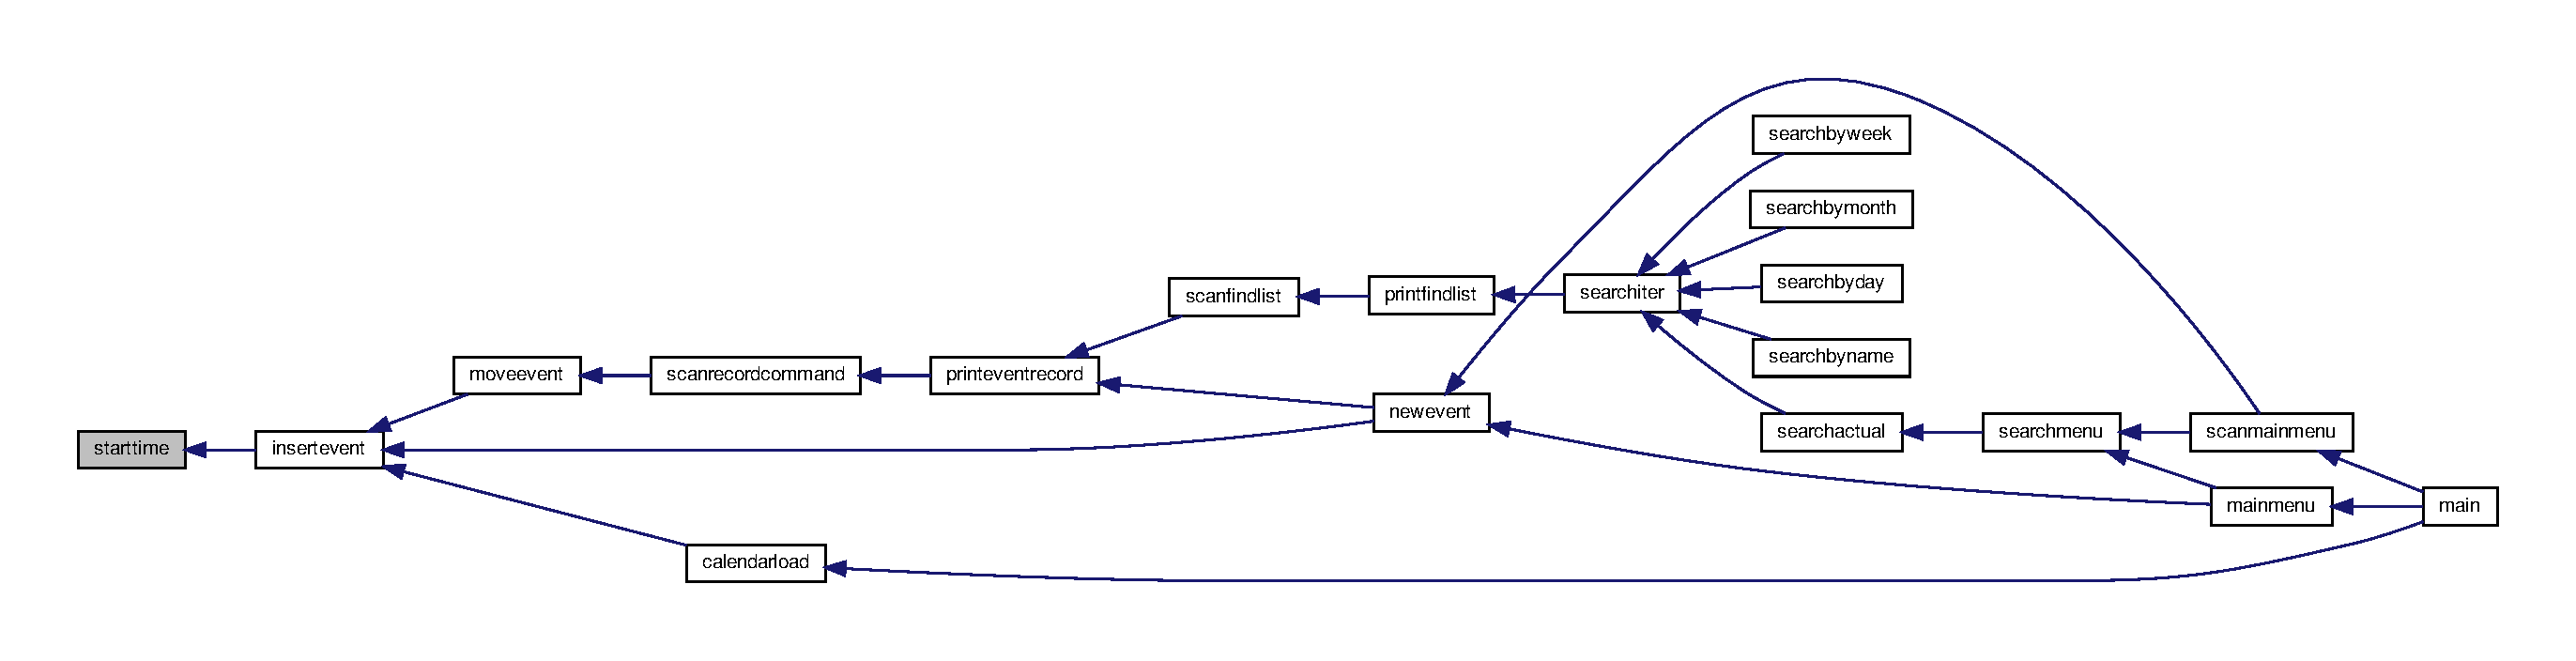
\includegraphics[width=350pt]{list_8c_a8f7708495c6e39bb6e712218711b331f_icgraph}
\end{center}
\end{figure}

\hypertarget{list_8h}{}\section{/home/dani/\+Documents/egyetem/prog1/nagyhazi/hazi2/calendar2/calendar/list.h File Reference}
\label{list_8h}\index{/home/dani/\+Documents/egyetem/prog1/nagyhazi/hazi2/calendar2/calendar/list.\+h@{/home/dani/\+Documents/egyetem/prog1/nagyhazi/hazi2/calendar2/calendar/list.\+h}}
{\ttfamily \#include \char`\"{}structures.\+h\char`\"{}}\newline
{\ttfamily \#include $<$time.\+h$>$}\newline
Include dependency graph for list.\+h\+:\nopagebreak
\begin{figure}[H]
\begin{center}
\leavevmode
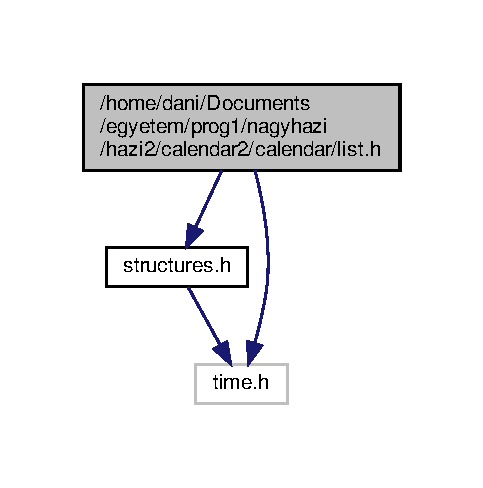
\includegraphics[width=232pt]{list_8h__incl}
\end{center}
\end{figure}
This graph shows which files directly or indirectly include this file\+:
\nopagebreak
\begin{figure}[H]
\begin{center}
\leavevmode
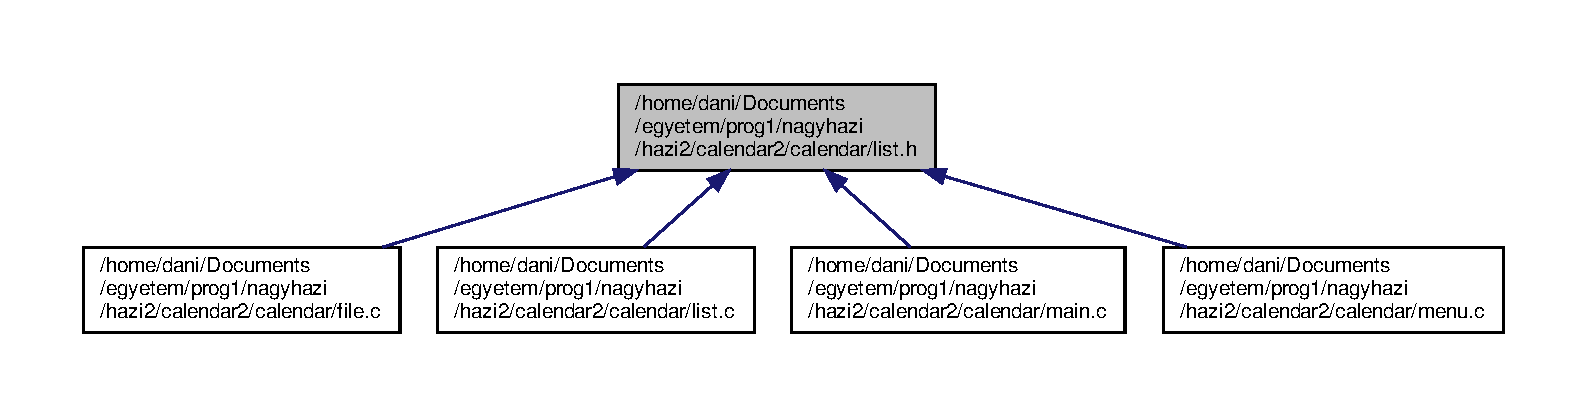
\includegraphics[width=350pt]{list_8h__dep__incl}
\end{center}
\end{figure}
\subsection*{Typedefs}
\begin{DoxyCompactItemize}
\item 
typedef struct tm \hyperlink{list_8h_affc453d30a4a6ce81ed778fd04d2d256}{Tm}
\end{DoxyCompactItemize}
\subsection*{Functions}
\begin{DoxyCompactItemize}
\item 
\hyperlink{struct_event_list}{Event\+List} $\ast$ \hyperlink{list_8h_a48f44148563512bd32274821f478bd1b}{initeventlist} ()
\item 
void \hyperlink{list_8h_a2561d96be1299fd3f5730c6d82143709}{printevent\+\_\+short} (\hyperlink{struct_event}{Event} $\ast$event)
\item 
void \hyperlink{list_8h_a7ef519287e473ee333204280a5d91403}{insertevent} (\hyperlink{struct_event_list}{Event\+List} $\ast$eventlist, \hyperlink{struct_event}{Event} $\ast$event)
\item 
\hyperlink{struct_event}{Event} $\ast$ \hyperlink{list_8h_a24fd1b37eee54600b66c42e86b52244a}{createevent} (int ev, int honap, int nap, int ora, int perc, int bora, int bperc, char $\ast$nev, char $\ast$hely, char $\ast$comment)
\end{DoxyCompactItemize}


\subsection{Typedef Documentation}
\mbox{\Hypertarget{list_8h_affc453d30a4a6ce81ed778fd04d2d256}\label{list_8h_affc453d30a4a6ce81ed778fd04d2d256}} 
\index{list.\+h@{list.\+h}!Tm@{Tm}}
\index{Tm@{Tm}!list.\+h@{list.\+h}}
\subsubsection{\texorpdfstring{Tm}{Tm}}
{\footnotesize\ttfamily typedef struct tm \hyperlink{list_8h_affc453d30a4a6ce81ed778fd04d2d256}{Tm}}



\subsection{Function Documentation}
\mbox{\Hypertarget{list_8h_a24fd1b37eee54600b66c42e86b52244a}\label{list_8h_a24fd1b37eee54600b66c42e86b52244a}} 
\index{list.\+h@{list.\+h}!createevent@{createevent}}
\index{createevent@{createevent}!list.\+h@{list.\+h}}
\subsubsection{\texorpdfstring{createevent()}{createevent()}}
{\footnotesize\ttfamily \hyperlink{struct_event}{Event}$\ast$ createevent (\begin{DoxyParamCaption}\item[{int}]{ev,  }\item[{int}]{honap,  }\item[{int}]{nap,  }\item[{int}]{ora,  }\item[{int}]{perc,  }\item[{int}]{bora,  }\item[{int}]{bperc,  }\item[{char $\ast$}]{nev,  }\item[{char $\ast$}]{hely,  }\item[{char $\ast$}]{comment }\end{DoxyParamCaption})}

Here is the caller graph for this function\+:
\nopagebreak
\begin{figure}[H]
\begin{center}
\leavevmode
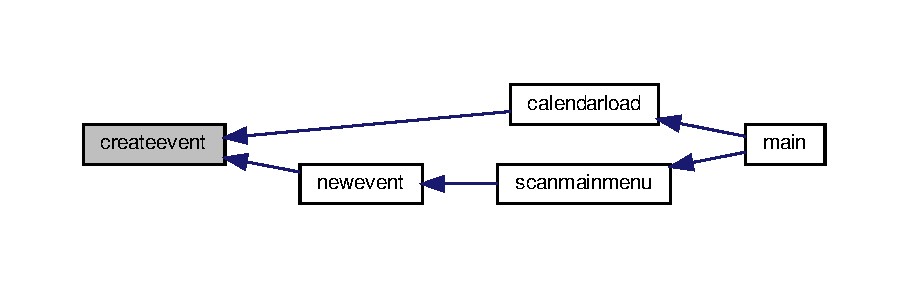
\includegraphics[width=350pt]{list_8h_a24fd1b37eee54600b66c42e86b52244a_icgraph}
\end{center}
\end{figure}
\mbox{\Hypertarget{list_8h_a48f44148563512bd32274821f478bd1b}\label{list_8h_a48f44148563512bd32274821f478bd1b}} 
\index{list.\+h@{list.\+h}!initeventlist@{initeventlist}}
\index{initeventlist@{initeventlist}!list.\+h@{list.\+h}}
\subsubsection{\texorpdfstring{initeventlist()}{initeventlist()}}
{\footnotesize\ttfamily \hyperlink{struct_event_list}{Event\+List}$\ast$ initeventlist (\begin{DoxyParamCaption}{ }\end{DoxyParamCaption})}

Here is the caller graph for this function\+:
\nopagebreak
\begin{figure}[H]
\begin{center}
\leavevmode
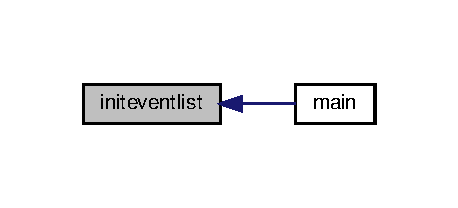
\includegraphics[width=220pt]{list_8h_a48f44148563512bd32274821f478bd1b_icgraph}
\end{center}
\end{figure}
\mbox{\Hypertarget{list_8h_a7ef519287e473ee333204280a5d91403}\label{list_8h_a7ef519287e473ee333204280a5d91403}} 
\index{list.\+h@{list.\+h}!insertevent@{insertevent}}
\index{insertevent@{insertevent}!list.\+h@{list.\+h}}
\subsubsection{\texorpdfstring{insertevent()}{insertevent()}}
{\footnotesize\ttfamily void insertevent (\begin{DoxyParamCaption}\item[{\hyperlink{struct_event_list}{Event\+List} $\ast$}]{eventlist,  }\item[{\hyperlink{struct_event}{Event} $\ast$}]{event }\end{DoxyParamCaption})}

Here is the call graph for this function\+:
\nopagebreak
\begin{figure}[H]
\begin{center}
\leavevmode
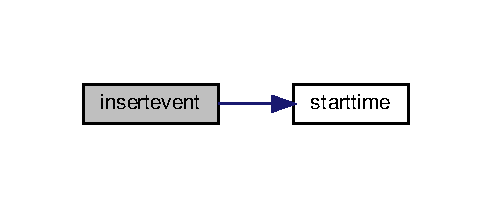
\includegraphics[width=236pt]{list_8h_a7ef519287e473ee333204280a5d91403_cgraph}
\end{center}
\end{figure}
Here is the caller graph for this function\+:
\nopagebreak
\begin{figure}[H]
\begin{center}
\leavevmode
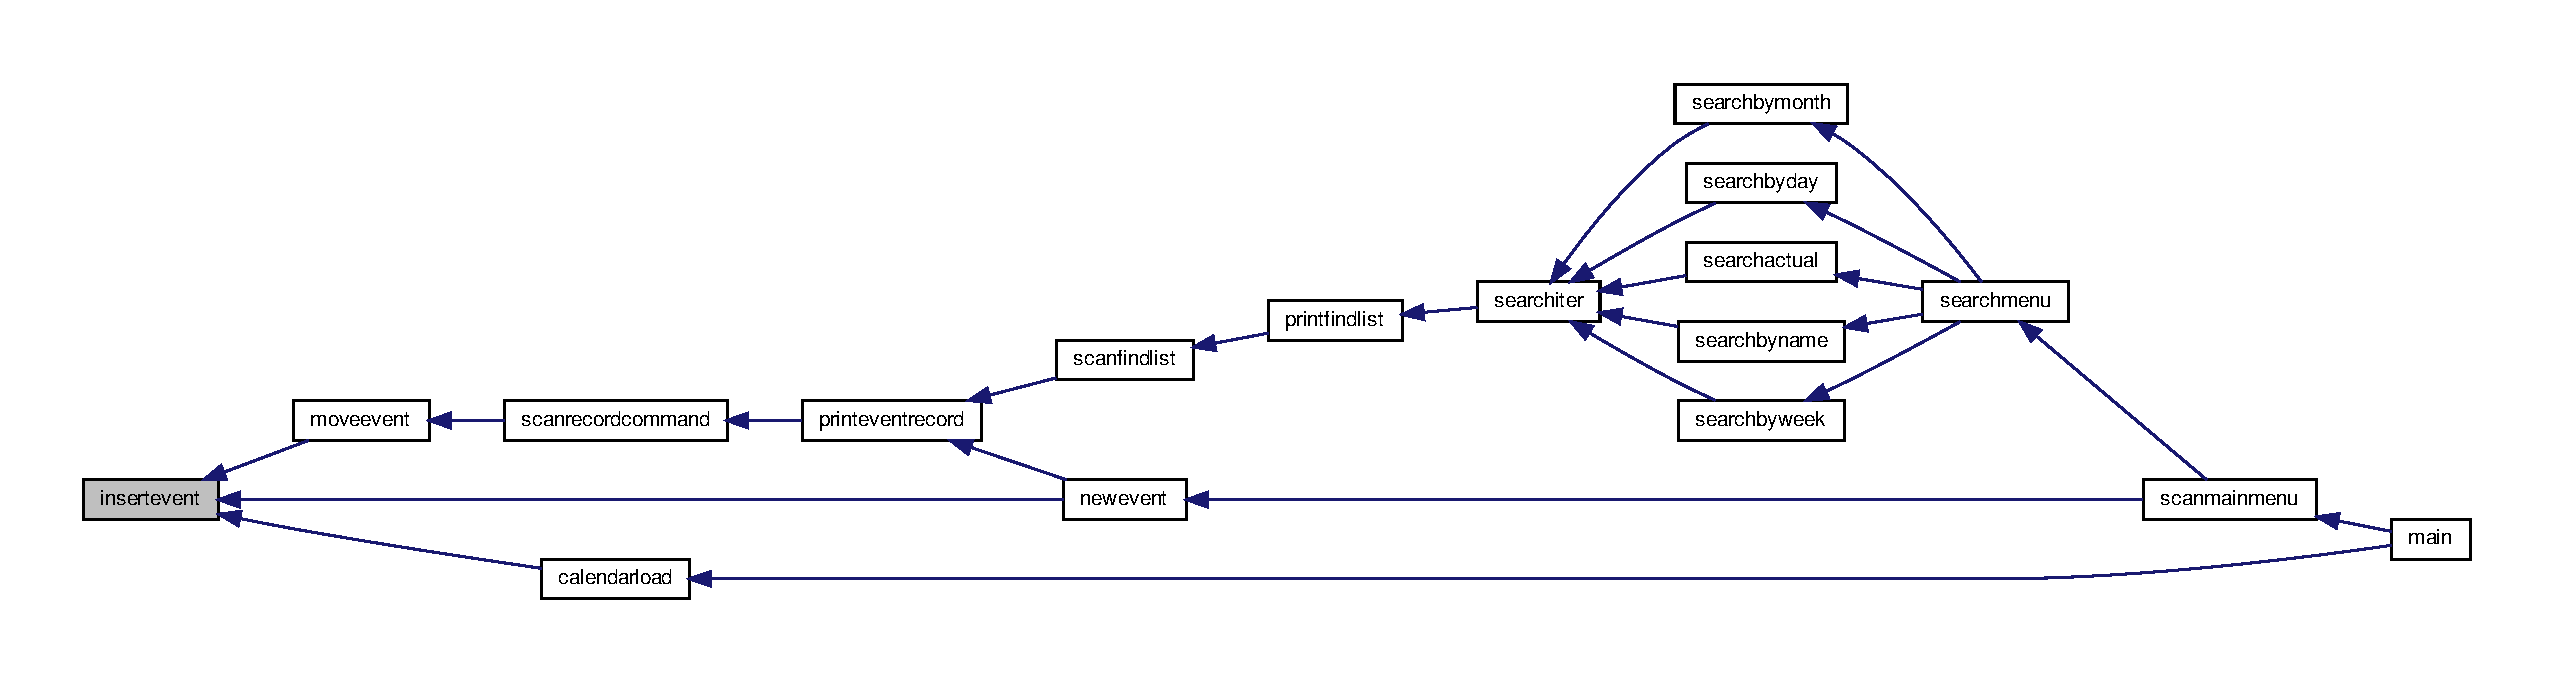
\includegraphics[width=350pt]{list_8h_a7ef519287e473ee333204280a5d91403_icgraph}
\end{center}
\end{figure}
\mbox{\Hypertarget{list_8h_a2561d96be1299fd3f5730c6d82143709}\label{list_8h_a2561d96be1299fd3f5730c6d82143709}} 
\index{list.\+h@{list.\+h}!printevent\+\_\+short@{printevent\+\_\+short}}
\index{printevent\+\_\+short@{printevent\+\_\+short}!list.\+h@{list.\+h}}
\subsubsection{\texorpdfstring{printevent\+\_\+short()}{printevent\_short()}}
{\footnotesize\ttfamily void printevent\+\_\+short (\begin{DoxyParamCaption}\item[{\hyperlink{struct_event}{Event} $\ast$}]{event }\end{DoxyParamCaption})}

Here is the caller graph for this function\+:
\nopagebreak
\begin{figure}[H]
\begin{center}
\leavevmode
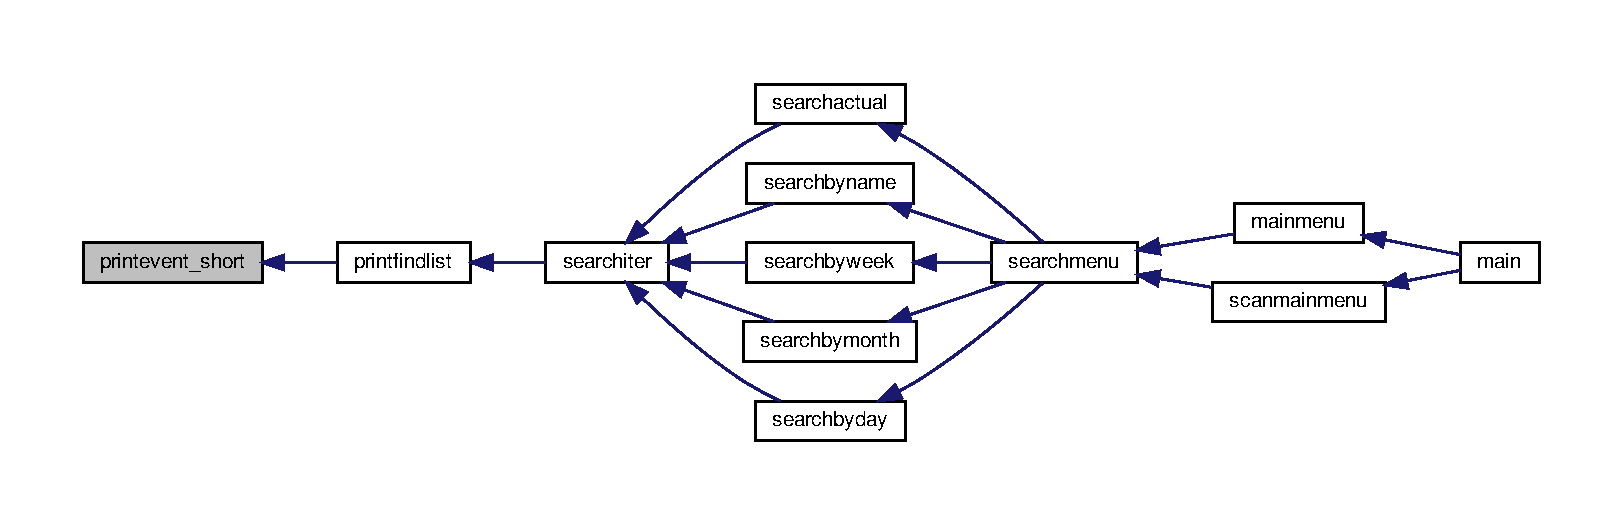
\includegraphics[width=350pt]{list_8h_a2561d96be1299fd3f5730c6d82143709_icgraph}
\end{center}
\end{figure}

\hypertarget{main_8c}{}\section{/home/dani/\+Documents/egyetem/prog1/nagyhazi/hazi2/calendar2/calendar/main.c File Reference}
\label{main_8c}\index{/home/dani/\+Documents/egyetem/prog1/nagyhazi/hazi2/calendar2/calendar/main.\+c@{/home/dani/\+Documents/egyetem/prog1/nagyhazi/hazi2/calendar2/calendar/main.\+c}}
{\ttfamily \#include $<$stdio.\+h$>$}\newline
{\ttfamily \#include $<$stdlib.\+h$>$}\newline
{\ttfamily \#include \char`\"{}structures.\+h\char`\"{}}\newline
{\ttfamily \#include \char`\"{}file.\+h\char`\"{}}\newline
{\ttfamily \#include \char`\"{}list.\+h\char`\"{}}\newline
{\ttfamily \#include \char`\"{}menu.\+h\char`\"{}}\newline
{\ttfamily \#include $<$stdbool.\+h$>$}\newline
{\ttfamily \#include \char`\"{}debugmalloc.\+h\char`\"{}}\newline
\subsection*{Functions}
\begin{DoxyCompactItemize}
\item 
int \hyperlink{main_8c_ae66f6b31b5ad750f1fe042a706a4e3d4}{main} ()
\end{DoxyCompactItemize}


\subsection{Function Documentation}
\mbox{\Hypertarget{main_8c_ae66f6b31b5ad750f1fe042a706a4e3d4}\label{main_8c_ae66f6b31b5ad750f1fe042a706a4e3d4}} 
\index{main.\+c@{main.\+c}!main@{main}}
\index{main@{main}!main.\+c@{main.\+c}}
\subsubsection{\texorpdfstring{main()}{main()}}
{\footnotesize\ttfamily int main (\begin{DoxyParamCaption}{ }\end{DoxyParamCaption})}


\hypertarget{menu_8c}{}\section{/home/dani/\+Documents/egyetem/prog1/nagyhazi/hazi2/calendar2/calendar/menu.c File Reference}
\label{menu_8c}\index{/home/dani/\+Documents/egyetem/prog1/nagyhazi/hazi2/calendar2/calendar/menu.\+c@{/home/dani/\+Documents/egyetem/prog1/nagyhazi/hazi2/calendar2/calendar/menu.\+c}}
{\ttfamily \#include \char`\"{}menu.\+h\char`\"{}}\newline
{\ttfamily \#include \char`\"{}structures.\+h\char`\"{}}\newline
{\ttfamily \#include $<$stdlib.\+h$>$}\newline
{\ttfamily \#include \char`\"{}file.\+h\char`\"{}}\newline
{\ttfamily \#include $<$stdio.\+h$>$}\newline
{\ttfamily \#include $<$string.\+h$>$}\newline
{\ttfamily \#include $<$stdbool.\+h$>$}\newline
Include dependency graph for menu.\+c\+:\nopagebreak
\begin{figure}[H]
\begin{center}
\leavevmode
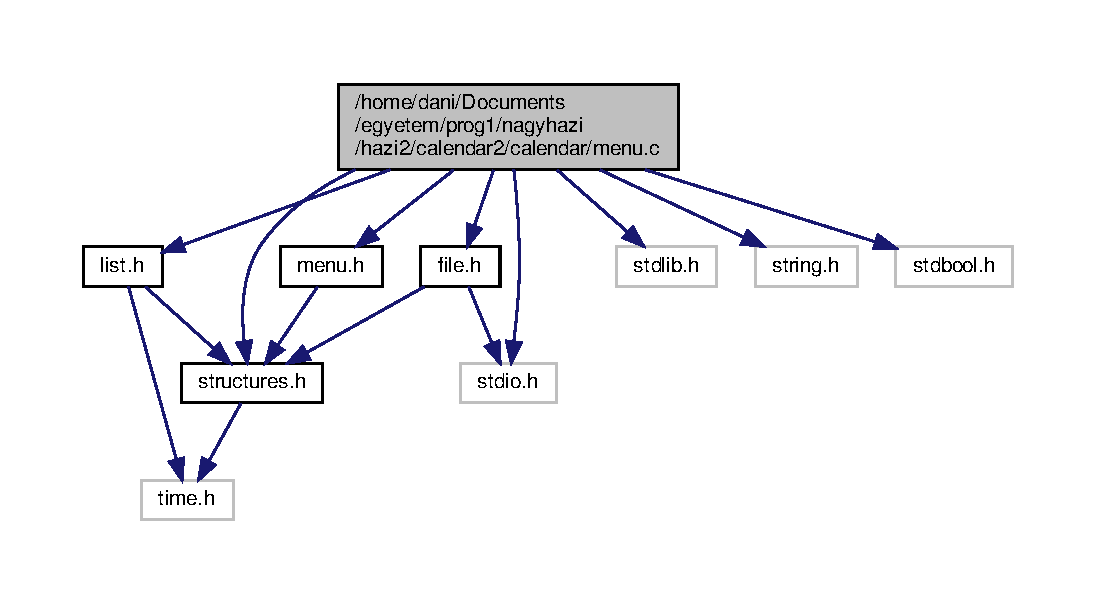
\includegraphics[width=350pt]{menu_8c__incl}
\end{center}
\end{figure}
\subsection*{Functions}
\begin{DoxyCompactItemize}
\item 
void \hyperlink{menu_8c_afc715bc6c0b9a9e85af15dc509a8d34b}{filesave} (\hyperlink{struct_event_list}{Event\+List} $\ast$eventlist)
\item 
void \hyperlink{menu_8c_ac2c3136ef241a7150d7cff391a0eb048}{newevent} (\hyperlink{struct_event_list}{Event\+List} $\ast$eventlist)
\item 
char $\ast$ \hyperlink{menu_8c_ab9ac014b764791c1dc71c187dca898f7}{hosszu\+\_\+sort\+\_\+olvas} (int bufferhossz)
\item 
void \hyperlink{menu_8c_ac86d3169260f5cacd0f792743957b054}{mainmenu} ()
\item 
void \hyperlink{menu_8c_a8e572ab27981dcd7144340fd25a24c80}{scanmainmenu} (\hyperlink{struct_event_list}{Event\+List} $\ast$eventlist)
\item 
void \hyperlink{menu_8c_a38d64ff02f60ebcb1988655ea12540a6}{searchmenu} (\hyperlink{struct_event_list}{Event\+List} $\ast$eventlist)
\item 
void \hyperlink{menu_8c_aa28daf84be098b64b8dfea8a88050f13}{savemenu} (\hyperlink{struct_event_list}{Event\+List} $\ast$eventlist)
\item 
int \hyperlink{menu_8c_a6ef5647864065ede4ef3b2773cbb9e8d}{scansavemenu} (\hyperlink{struct_event_list}{Event\+List} $\ast$eventlist)
\item 
void \hyperlink{menu_8c_ac651d3838f4da7bf6055fa839621e289}{exitmenu} (\hyperlink{struct_event_list}{Event\+List} $\ast$eventlist)
\item 
int \hyperlink{menu_8c_aa12eba16d2e2bd5dfc70240d19bd5c8e}{scanexitmenu} (\hyperlink{struct_event_list}{Event\+List} $\ast$eventlist)
\item 
int \hyperlink{menu_8c_a1aa7ba6b6941a272c34eea491e4a650d}{printmenu} (\hyperlink{struct_menu_pont}{Menu\+Pont} $\ast$menupontok)
\item 
void \hyperlink{menu_8c_a00af175f266f31d352be878cfb5d5640}{callmenu} (int meret, \hyperlink{struct_menu_pont}{Menu\+Pont} $\ast$menupontok, \hyperlink{struct_event_list}{Event\+List} $\ast$eventlist)
\end{DoxyCompactItemize}


\subsection{Function Documentation}
\mbox{\Hypertarget{menu_8c_a00af175f266f31d352be878cfb5d5640}\label{menu_8c_a00af175f266f31d352be878cfb5d5640}} 
\index{menu.\+c@{menu.\+c}!callmenu@{callmenu}}
\index{callmenu@{callmenu}!menu.\+c@{menu.\+c}}
\subsubsection{\texorpdfstring{callmenu()}{callmenu()}}
{\footnotesize\ttfamily void callmenu (\begin{DoxyParamCaption}\item[{int}]{meret,  }\item[{\hyperlink{struct_menu_pont}{Menu\+Pont} $\ast$}]{menupontok,  }\item[{\hyperlink{struct_event_list}{Event\+List} $\ast$}]{eventlist }\end{DoxyParamCaption})}

\mbox{\Hypertarget{menu_8c_ac651d3838f4da7bf6055fa839621e289}\label{menu_8c_ac651d3838f4da7bf6055fa839621e289}} 
\index{menu.\+c@{menu.\+c}!exitmenu@{exitmenu}}
\index{exitmenu@{exitmenu}!menu.\+c@{menu.\+c}}
\subsubsection{\texorpdfstring{exitmenu()}{exitmenu()}}
{\footnotesize\ttfamily void exitmenu (\begin{DoxyParamCaption}\item[{\hyperlink{struct_event_list}{Event\+List} $\ast$}]{eventlist }\end{DoxyParamCaption})}

Here is the call graph for this function\+:\nopagebreak
\begin{figure}[H]
\begin{center}
\leavevmode
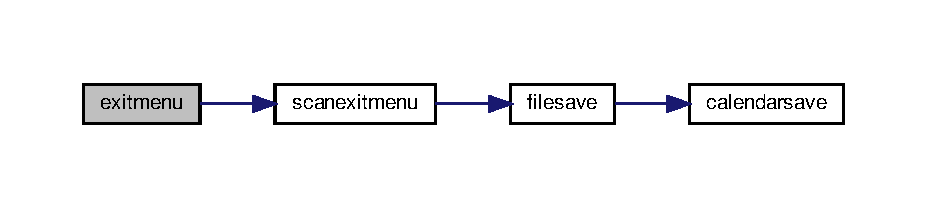
\includegraphics[width=335pt]{menu_8c_ac651d3838f4da7bf6055fa839621e289_cgraph}
\end{center}
\end{figure}
Here is the caller graph for this function\+:
\nopagebreak
\begin{figure}[H]
\begin{center}
\leavevmode
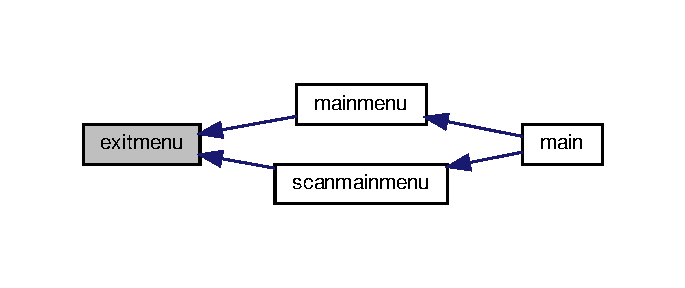
\includegraphics[width=329pt]{menu_8c_ac651d3838f4da7bf6055fa839621e289_icgraph}
\end{center}
\end{figure}
\mbox{\Hypertarget{menu_8c_afc715bc6c0b9a9e85af15dc509a8d34b}\label{menu_8c_afc715bc6c0b9a9e85af15dc509a8d34b}} 
\index{menu.\+c@{menu.\+c}!filesave@{filesave}}
\index{filesave@{filesave}!menu.\+c@{menu.\+c}}
\subsubsection{\texorpdfstring{filesave()}{filesave()}}
{\footnotesize\ttfamily void filesave (\begin{DoxyParamCaption}\item[{\hyperlink{struct_event_list}{Event\+List} $\ast$}]{eventlist }\end{DoxyParamCaption})}

Here is the caller graph for this function\+:
\nopagebreak
\begin{figure}[H]
\begin{center}
\leavevmode
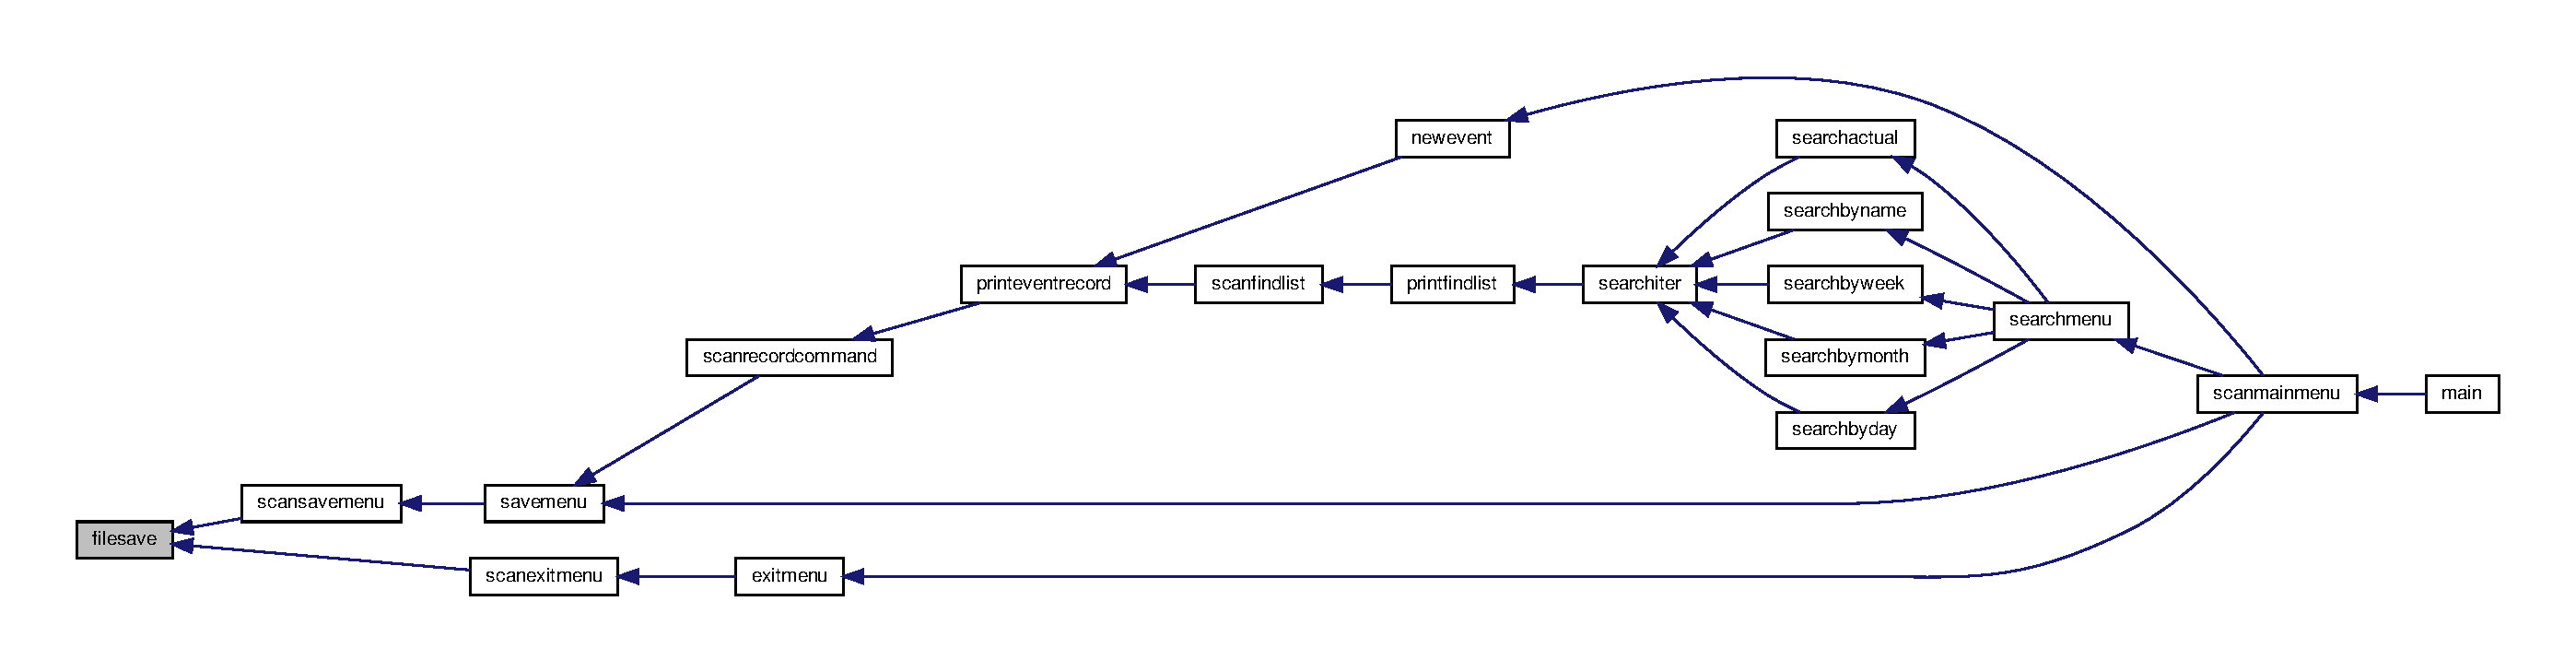
\includegraphics[width=350pt]{menu_8c_afc715bc6c0b9a9e85af15dc509a8d34b_icgraph}
\end{center}
\end{figure}
\mbox{\Hypertarget{menu_8c_ab9ac014b764791c1dc71c187dca898f7}\label{menu_8c_ab9ac014b764791c1dc71c187dca898f7}} 
\index{menu.\+c@{menu.\+c}!hosszu\+\_\+sort\+\_\+olvas@{hosszu\+\_\+sort\+\_\+olvas}}
\index{hosszu\+\_\+sort\+\_\+olvas@{hosszu\+\_\+sort\+\_\+olvas}!menu.\+c@{menu.\+c}}
\subsubsection{\texorpdfstring{hosszu\+\_\+sort\+\_\+olvas()}{hosszu\_sort\_olvas()}}
{\footnotesize\ttfamily char$\ast$ hosszu\+\_\+sort\+\_\+olvas (\begin{DoxyParamCaption}\item[{int}]{bufferhossz }\end{DoxyParamCaption})}

\mbox{\Hypertarget{menu_8c_ac86d3169260f5cacd0f792743957b054}\label{menu_8c_ac86d3169260f5cacd0f792743957b054}} 
\index{menu.\+c@{menu.\+c}!mainmenu@{mainmenu}}
\index{mainmenu@{mainmenu}!menu.\+c@{menu.\+c}}
\subsubsection{\texorpdfstring{mainmenu()}{mainmenu()}}
{\footnotesize\ttfamily void mainmenu (\begin{DoxyParamCaption}{ }\end{DoxyParamCaption})}

Here is the call graph for this function\+:
\nopagebreak
\begin{figure}[H]
\begin{center}
\leavevmode
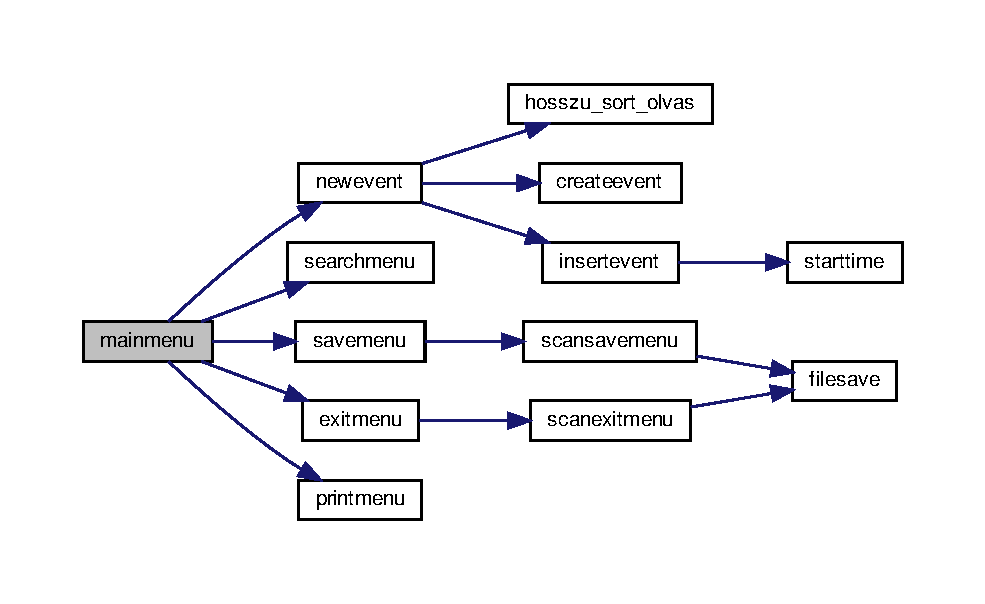
\includegraphics[width=350pt]{menu_8c_ac86d3169260f5cacd0f792743957b054_cgraph}
\end{center}
\end{figure}
Here is the caller graph for this function\+:
\nopagebreak
\begin{figure}[H]
\begin{center}
\leavevmode
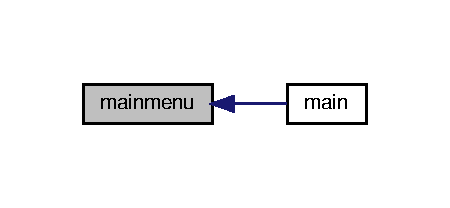
\includegraphics[width=216pt]{menu_8c_ac86d3169260f5cacd0f792743957b054_icgraph}
\end{center}
\end{figure}
\mbox{\Hypertarget{menu_8c_ac2c3136ef241a7150d7cff391a0eb048}\label{menu_8c_ac2c3136ef241a7150d7cff391a0eb048}} 
\index{menu.\+c@{menu.\+c}!newevent@{newevent}}
\index{newevent@{newevent}!menu.\+c@{menu.\+c}}
\subsubsection{\texorpdfstring{newevent()}{newevent()}}
{\footnotesize\ttfamily void newevent (\begin{DoxyParamCaption}\item[{\hyperlink{struct_event_list}{Event\+List} $\ast$}]{eventlist }\end{DoxyParamCaption})}

Here is the call graph for this function\+:
\nopagebreak
\begin{figure}[H]
\begin{center}
\leavevmode
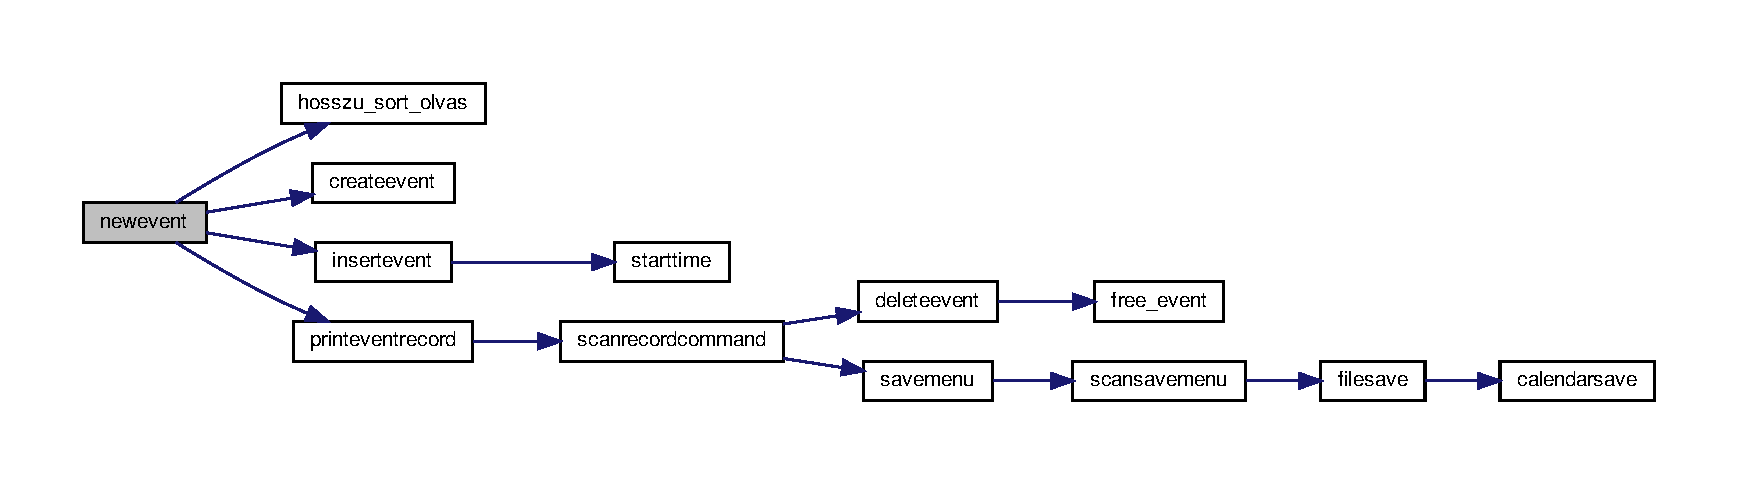
\includegraphics[width=240pt]{menu_8c_ac2c3136ef241a7150d7cff391a0eb048_cgraph}
\end{center}
\end{figure}
Here is the caller graph for this function\+:
\nopagebreak
\begin{figure}[H]
\begin{center}
\leavevmode
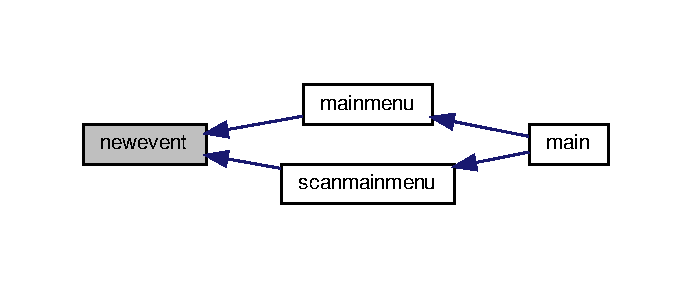
\includegraphics[width=332pt]{menu_8c_ac2c3136ef241a7150d7cff391a0eb048_icgraph}
\end{center}
\end{figure}
\mbox{\Hypertarget{menu_8c_a1aa7ba6b6941a272c34eea491e4a650d}\label{menu_8c_a1aa7ba6b6941a272c34eea491e4a650d}} 
\index{menu.\+c@{menu.\+c}!printmenu@{printmenu}}
\index{printmenu@{printmenu}!menu.\+c@{menu.\+c}}
\subsubsection{\texorpdfstring{printmenu()}{printmenu()}}
{\footnotesize\ttfamily int printmenu (\begin{DoxyParamCaption}\item[{\hyperlink{struct_menu_pont}{Menu\+Pont} $\ast$}]{menupontok }\end{DoxyParamCaption})}

Here is the caller graph for this function\+:
\nopagebreak
\begin{figure}[H]
\begin{center}
\leavevmode
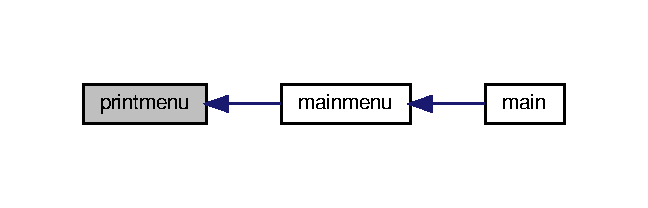
\includegraphics[width=311pt]{menu_8c_a1aa7ba6b6941a272c34eea491e4a650d_icgraph}
\end{center}
\end{figure}
\mbox{\Hypertarget{menu_8c_aa28daf84be098b64b8dfea8a88050f13}\label{menu_8c_aa28daf84be098b64b8dfea8a88050f13}} 
\index{menu.\+c@{menu.\+c}!savemenu@{savemenu}}
\index{savemenu@{savemenu}!menu.\+c@{menu.\+c}}
\subsubsection{\texorpdfstring{savemenu()}{savemenu()}}
{\footnotesize\ttfamily void savemenu (\begin{DoxyParamCaption}\item[{\hyperlink{struct_event_list}{Event\+List} $\ast$}]{eventlist }\end{DoxyParamCaption})}

Here is the call graph for this function\+:
\nopagebreak
\begin{figure}[H]
\begin{center}
\leavevmode
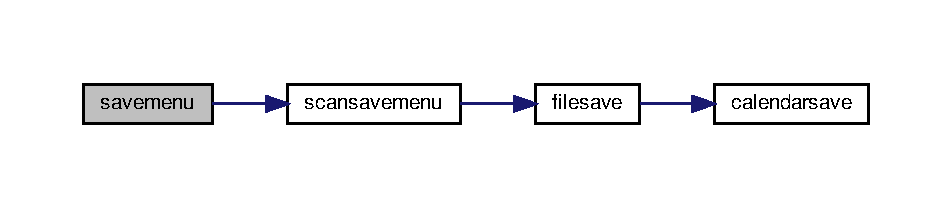
\includegraphics[width=347pt]{menu_8c_aa28daf84be098b64b8dfea8a88050f13_cgraph}
\end{center}
\end{figure}
Here is the caller graph for this function\+:
\nopagebreak
\begin{figure}[H]
\begin{center}
\leavevmode
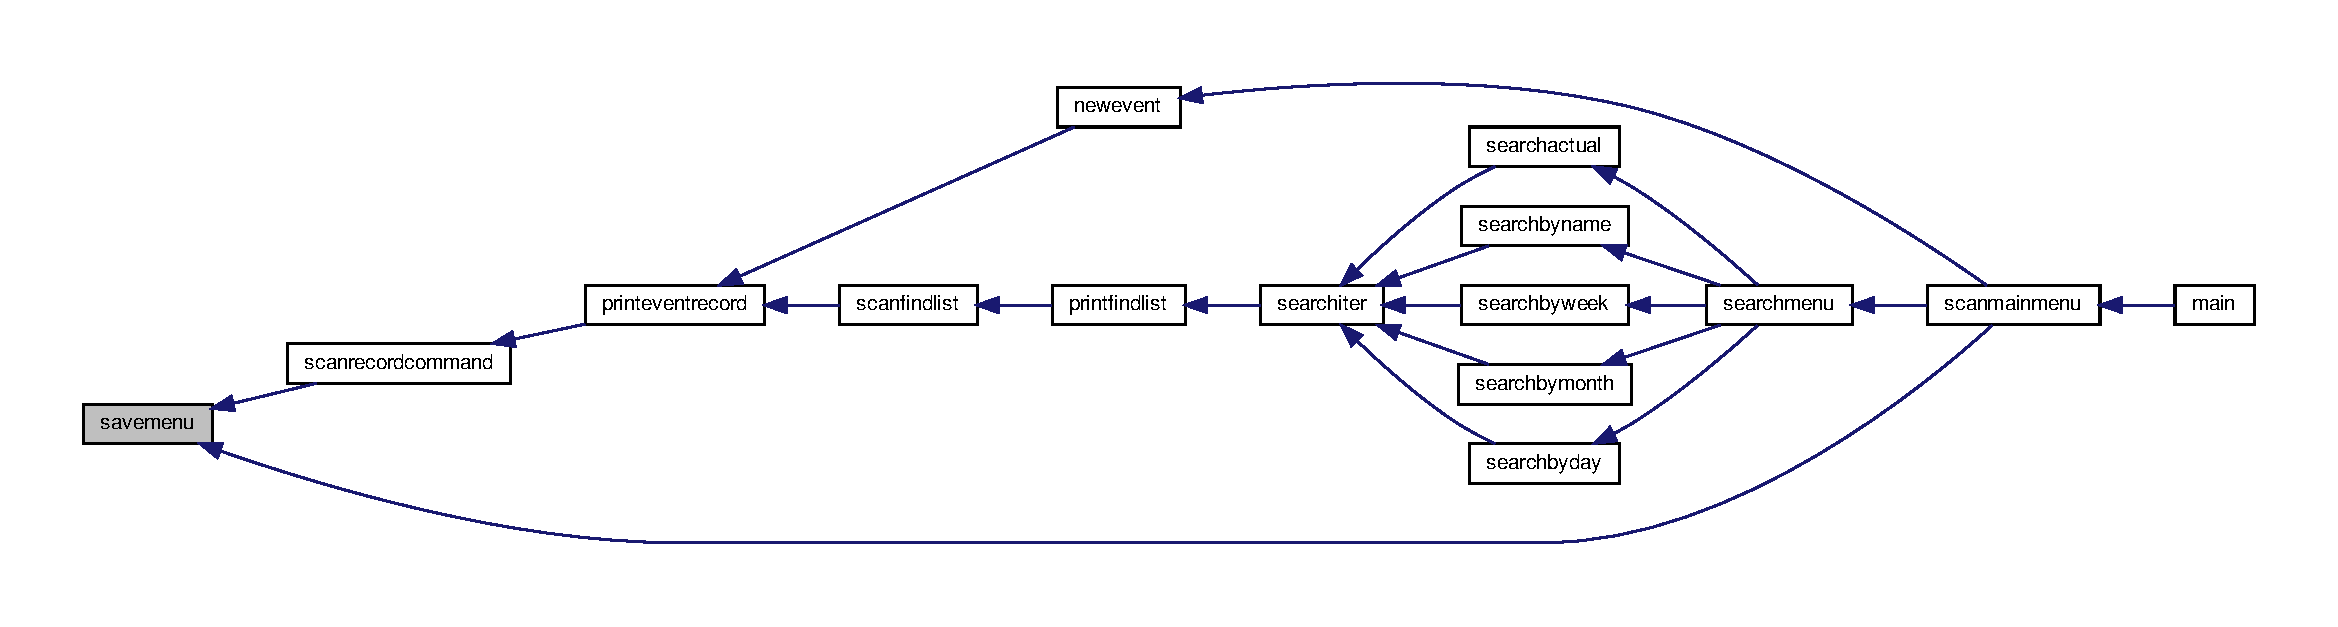
\includegraphics[width=335pt]{menu_8c_aa28daf84be098b64b8dfea8a88050f13_icgraph}
\end{center}
\end{figure}
\mbox{\Hypertarget{menu_8c_aa12eba16d2e2bd5dfc70240d19bd5c8e}\label{menu_8c_aa12eba16d2e2bd5dfc70240d19bd5c8e}} 
\index{menu.\+c@{menu.\+c}!scanexitmenu@{scanexitmenu}}
\index{scanexitmenu@{scanexitmenu}!menu.\+c@{menu.\+c}}
\subsubsection{\texorpdfstring{scanexitmenu()}{scanexitmenu()}}
{\footnotesize\ttfamily int scanexitmenu (\begin{DoxyParamCaption}\item[{\hyperlink{struct_event_list}{Event\+List} $\ast$}]{eventlist }\end{DoxyParamCaption})}

Here is the call graph for this function\+:
\nopagebreak
\begin{figure}[H]
\begin{center}
\leavevmode
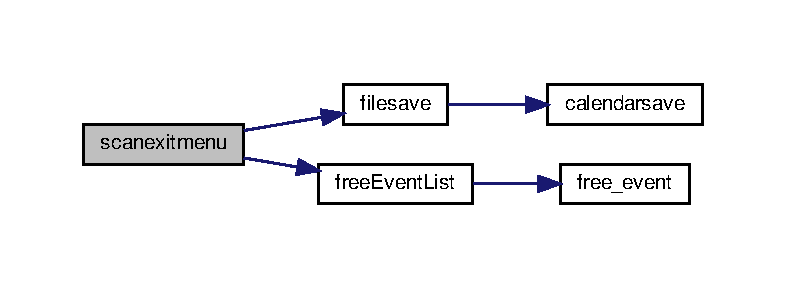
\includegraphics[width=243pt]{menu_8c_aa12eba16d2e2bd5dfc70240d19bd5c8e_cgraph}
\end{center}
\end{figure}
Here is the caller graph for this function\+:
\nopagebreak
\begin{figure}[H]
\begin{center}
\leavevmode
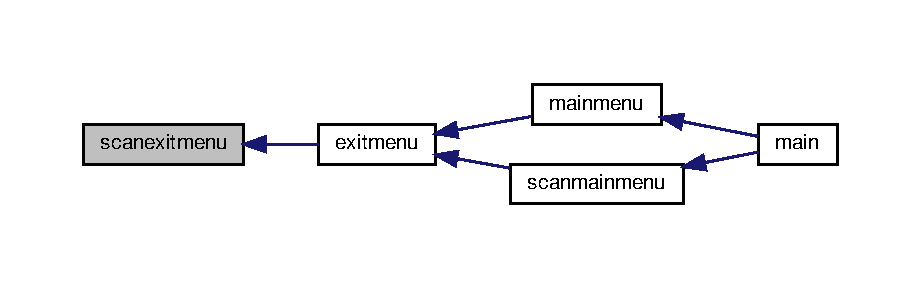
\includegraphics[width=350pt]{menu_8c_aa12eba16d2e2bd5dfc70240d19bd5c8e_icgraph}
\end{center}
\end{figure}
\mbox{\Hypertarget{menu_8c_a8e572ab27981dcd7144340fd25a24c80}\label{menu_8c_a8e572ab27981dcd7144340fd25a24c80}} 
\index{menu.\+c@{menu.\+c}!scanmainmenu@{scanmainmenu}}
\index{scanmainmenu@{scanmainmenu}!menu.\+c@{menu.\+c}}
\subsubsection{\texorpdfstring{scanmainmenu()}{scanmainmenu()}}
{\footnotesize\ttfamily void scanmainmenu (\begin{DoxyParamCaption}\item[{\hyperlink{struct_event_list}{Event\+List} $\ast$}]{eventlist }\end{DoxyParamCaption})}

Here is the call graph for this function\+:
\nopagebreak
\begin{figure}[H]
\begin{center}
\leavevmode
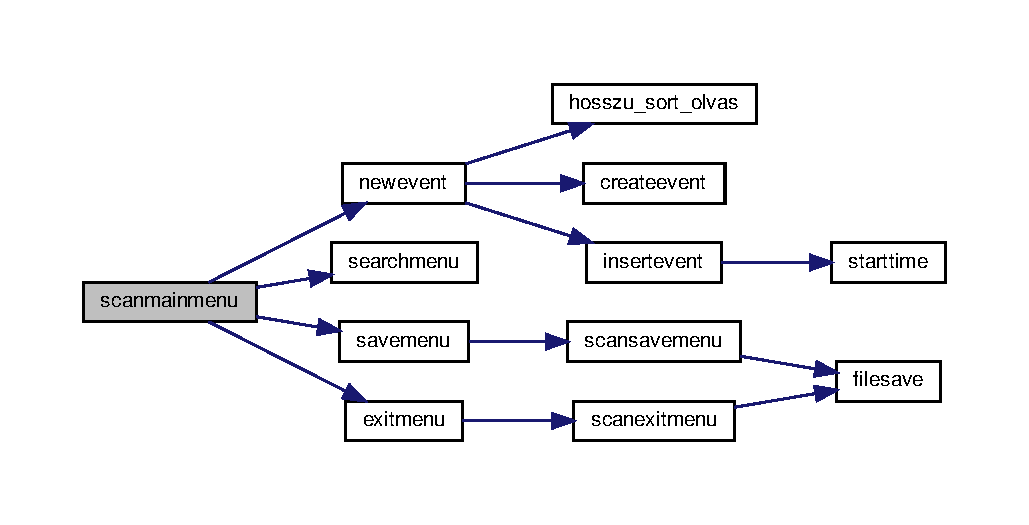
\includegraphics[width=350pt]{menu_8c_a8e572ab27981dcd7144340fd25a24c80_cgraph}
\end{center}
\end{figure}
Here is the caller graph for this function\+:
\nopagebreak
\begin{figure}[H]
\begin{center}
\leavevmode
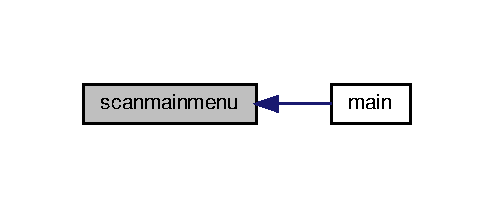
\includegraphics[width=237pt]{menu_8c_a8e572ab27981dcd7144340fd25a24c80_icgraph}
\end{center}
\end{figure}
\mbox{\Hypertarget{menu_8c_a6ef5647864065ede4ef3b2773cbb9e8d}\label{menu_8c_a6ef5647864065ede4ef3b2773cbb9e8d}} 
\index{menu.\+c@{menu.\+c}!scansavemenu@{scansavemenu}}
\index{scansavemenu@{scansavemenu}!menu.\+c@{menu.\+c}}
\subsubsection{\texorpdfstring{scansavemenu()}{scansavemenu()}}
{\footnotesize\ttfamily int scansavemenu (\begin{DoxyParamCaption}\item[{\hyperlink{struct_event_list}{Event\+List} $\ast$}]{eventlist }\end{DoxyParamCaption})}

Here is the call graph for this function\+:
\nopagebreak
\begin{figure}[H]
\begin{center}
\leavevmode
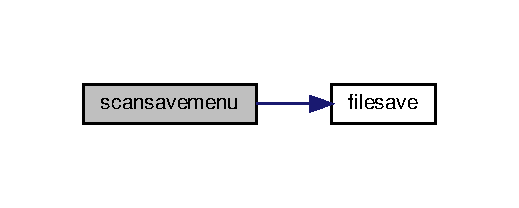
\includegraphics[width=249pt]{menu_8c_a6ef5647864065ede4ef3b2773cbb9e8d_cgraph}
\end{center}
\end{figure}
Here is the caller graph for this function\+:
\nopagebreak
\begin{figure}[H]
\begin{center}
\leavevmode
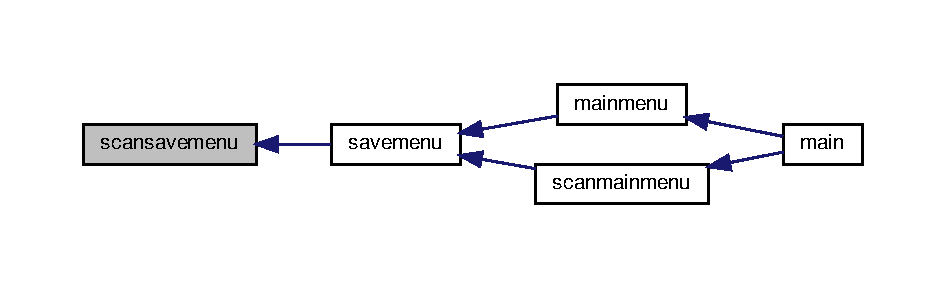
\includegraphics[width=350pt]{menu_8c_a6ef5647864065ede4ef3b2773cbb9e8d_icgraph}
\end{center}
\end{figure}
\mbox{\Hypertarget{menu_8c_a38d64ff02f60ebcb1988655ea12540a6}\label{menu_8c_a38d64ff02f60ebcb1988655ea12540a6}} 
\index{menu.\+c@{menu.\+c}!searchmenu@{searchmenu}}
\index{searchmenu@{searchmenu}!menu.\+c@{menu.\+c}}
\subsubsection{\texorpdfstring{searchmenu()}{searchmenu()}}
{\footnotesize\ttfamily void searchmenu (\begin{DoxyParamCaption}\item[{\hyperlink{struct_event_list}{Event\+List} $\ast$}]{eventlist }\end{DoxyParamCaption})}

Here is the caller graph for this function\+:
\nopagebreak
\begin{figure}[H]
\begin{center}
\leavevmode
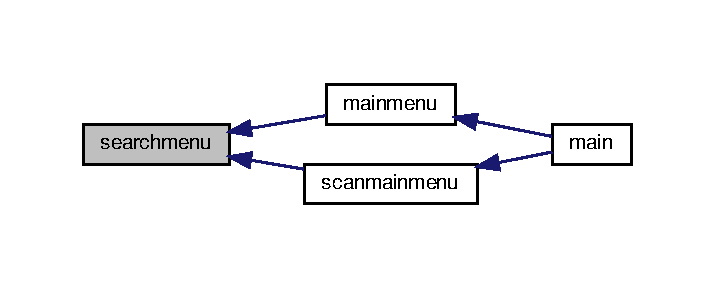
\includegraphics[width=343pt]{menu_8c_a38d64ff02f60ebcb1988655ea12540a6_icgraph}
\end{center}
\end{figure}

\hypertarget{menu_8h}{}\section{/home/dani/\+Documents/egyetem/prog1/nagyhazi/hazi2/calendar2/calendar/menu.h File Reference}
\label{menu_8h}\index{/home/dani/\+Documents/egyetem/prog1/nagyhazi/hazi2/calendar2/calendar/menu.\+h@{/home/dani/\+Documents/egyetem/prog1/nagyhazi/hazi2/calendar2/calendar/menu.\+h}}
{\ttfamily \#include \char`\"{}structures.\+h\char`\"{}}\newline
Include dependency graph for menu.\+h\+:
\nopagebreak
\begin{figure}[H]
\begin{center}
\leavevmode
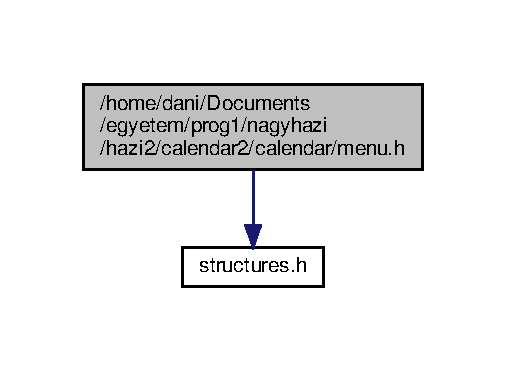
\includegraphics[width=243pt]{menu_8h__incl}
\end{center}
\end{figure}
This graph shows which files directly or indirectly include this file\+:
\nopagebreak
\begin{figure}[H]
\begin{center}
\leavevmode
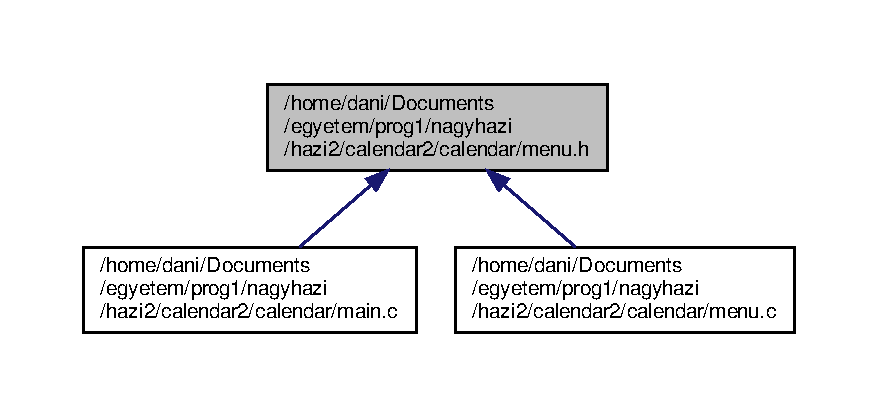
\includegraphics[width=350pt]{menu_8h__dep__incl}
\end{center}
\end{figure}
\subsection*{Functions}
\begin{DoxyCompactItemize}
\item 
void \hyperlink{menu_8h_a3fdfc75c2b95c21791f612f12c5a375d}{newevent} ()
\item 
void \hyperlink{menu_8h_a10d0e656ac5ff3a51135fee280274efa}{searchmenu} ()
\item 
void \hyperlink{menu_8h_a928aa131670ac3515aaacdeebb3e278a}{savemenu} ()
\item 
void \hyperlink{menu_8h_ada5bc1a6285c236343ce8a43ac9ab6cc}{exitmenu} ()
\item 
int \hyperlink{menu_8h_a1aa7ba6b6941a272c34eea491e4a650d}{printmenu} (\hyperlink{struct_menu_pont}{Menu\+Pont} $\ast$menupontok)
\item 
char $\ast$ \hyperlink{menu_8h_ab9ac014b764791c1dc71c187dca898f7}{hosszu\+\_\+sort\+\_\+olvas} (int bufferhossz)
\end{DoxyCompactItemize}


\subsection{Function Documentation}
\mbox{\Hypertarget{menu_8h_ada5bc1a6285c236343ce8a43ac9ab6cc}\label{menu_8h_ada5bc1a6285c236343ce8a43ac9ab6cc}} 
\index{menu.\+h@{menu.\+h}!exitmenu@{exitmenu}}
\index{exitmenu@{exitmenu}!menu.\+h@{menu.\+h}}
\subsubsection{\texorpdfstring{exitmenu()}{exitmenu()}}
{\footnotesize\ttfamily void exitmenu (\begin{DoxyParamCaption}{ }\end{DoxyParamCaption})}

\mbox{\Hypertarget{menu_8h_ab9ac014b764791c1dc71c187dca898f7}\label{menu_8h_ab9ac014b764791c1dc71c187dca898f7}} 
\index{menu.\+h@{menu.\+h}!hosszu\+\_\+sort\+\_\+olvas@{hosszu\+\_\+sort\+\_\+olvas}}
\index{hosszu\+\_\+sort\+\_\+olvas@{hosszu\+\_\+sort\+\_\+olvas}!menu.\+h@{menu.\+h}}
\subsubsection{\texorpdfstring{hosszu\+\_\+sort\+\_\+olvas()}{hosszu\_sort\_olvas()}}
{\footnotesize\ttfamily char$\ast$ hosszu\+\_\+sort\+\_\+olvas (\begin{DoxyParamCaption}\item[{int}]{bufferhossz }\end{DoxyParamCaption})}

Here is the caller graph for this function\+:
\nopagebreak
\begin{figure}[H]
\begin{center}
\leavevmode
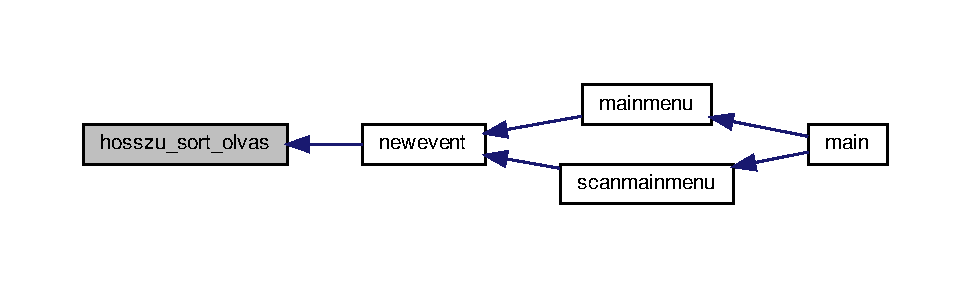
\includegraphics[width=350pt]{menu_8h_ab9ac014b764791c1dc71c187dca898f7_icgraph}
\end{center}
\end{figure}
\mbox{\Hypertarget{menu_8h_a3fdfc75c2b95c21791f612f12c5a375d}\label{menu_8h_a3fdfc75c2b95c21791f612f12c5a375d}} 
\index{menu.\+h@{menu.\+h}!newevent@{newevent}}
\index{newevent@{newevent}!menu.\+h@{menu.\+h}}
\subsubsection{\texorpdfstring{newevent()}{newevent()}}
{\footnotesize\ttfamily void newevent (\begin{DoxyParamCaption}{ }\end{DoxyParamCaption})}

\mbox{\Hypertarget{menu_8h_a1aa7ba6b6941a272c34eea491e4a650d}\label{menu_8h_a1aa7ba6b6941a272c34eea491e4a650d}} 
\index{menu.\+h@{menu.\+h}!printmenu@{printmenu}}
\index{printmenu@{printmenu}!menu.\+h@{menu.\+h}}
\subsubsection{\texorpdfstring{printmenu()}{printmenu()}}
{\footnotesize\ttfamily int printmenu (\begin{DoxyParamCaption}\item[{\hyperlink{struct_menu_pont}{Menu\+Pont} $\ast$}]{menupontok }\end{DoxyParamCaption})}

Here is the caller graph for this function\+:
\nopagebreak
\begin{figure}[H]
\begin{center}
\leavevmode
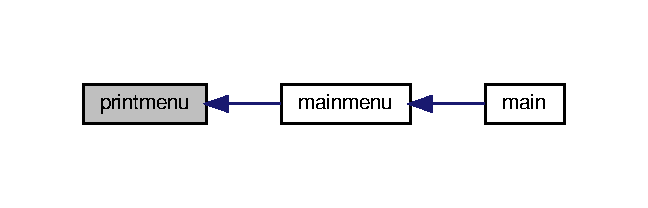
\includegraphics[width=311pt]{menu_8h_a1aa7ba6b6941a272c34eea491e4a650d_icgraph}
\end{center}
\end{figure}
\mbox{\Hypertarget{menu_8h_a928aa131670ac3515aaacdeebb3e278a}\label{menu_8h_a928aa131670ac3515aaacdeebb3e278a}} 
\index{menu.\+h@{menu.\+h}!savemenu@{savemenu}}
\index{savemenu@{savemenu}!menu.\+h@{menu.\+h}}
\subsubsection{\texorpdfstring{savemenu()}{savemenu()}}
{\footnotesize\ttfamily void savemenu (\begin{DoxyParamCaption}{ }\end{DoxyParamCaption})}

\mbox{\Hypertarget{menu_8h_a10d0e656ac5ff3a51135fee280274efa}\label{menu_8h_a10d0e656ac5ff3a51135fee280274efa}} 
\index{menu.\+h@{menu.\+h}!searchmenu@{searchmenu}}
\index{searchmenu@{searchmenu}!menu.\+h@{menu.\+h}}
\subsubsection{\texorpdfstring{searchmenu()}{searchmenu()}}
{\footnotesize\ttfamily void searchmenu (\begin{DoxyParamCaption}{ }\end{DoxyParamCaption})}


\hypertarget{search_8c}{}\section{/home/dani/\+Documents/egyetem/prog1/nagyhazi/hazi2/calendar2/calendar/search.c File Reference}
\label{search_8c}\index{/home/dani/\+Documents/egyetem/prog1/nagyhazi/hazi2/calendar2/calendar/search.\+c@{/home/dani/\+Documents/egyetem/prog1/nagyhazi/hazi2/calendar2/calendar/search.\+c}}
{\ttfamily \#include \char`\"{}search.\+h\char`\"{}}\newline
{\ttfamily \#include \char`\"{}structures.\+h\char`\"{}}\newline
{\ttfamily \#include $<$stdlib.\+h$>$}\newline
{\ttfamily \#include $<$string.\+h$>$}\newline
{\ttfamily \#include $<$stdbool.\+h$>$}\newline
{\ttfamily \#include $<$time.\+h$>$}\newline
{\ttfamily \#include $<$stdio.\+h$>$}\newline
{\ttfamily \#include \char`\"{}searchui.\+h\char`\"{}}\newline
\subsection*{Functions}
\begin{DoxyCompactItemize}
\item 
int \hyperlink{group__search_ga199722ea7869f598848648238f88d274}{searchiter} (\hyperlink{struct_event_list}{Event\+List} $\ast$eventlist, \hyperlink{struct_search_conditions}{Search\+Conditions} condition)
\item 
int \hyperlink{group__search_ga9a7e3230097d2f97a58082ff6eb864ac}{searchactual} (\hyperlink{struct_event_list}{Event\+List} $\ast$eventlist, \hyperlink{group__search_gaf9df49b17c9441844cafc15064ec50fc}{Search\+By} searchmode)
\item 
void \hyperlink{group__search_gace601ce27f555e73988b2db946d1ca5e}{inserttofindlist} (\hyperlink{struct_find_list}{Find\+List} $\ast$findlist, \hyperlink{struct_event}{Event} $\ast$event)
\item 
int \hyperlink{group__search_ga4e80bfd47c2fef45e9f6f50632544931}{tmtoweek} (\hyperlink{group__list_gaffc453d30a4a6ce81ed778fd04d2d256}{Tm} $\ast$tm)
\item 
\hyperlink{group__list_gaffc453d30a4a6ce81ed778fd04d2d256}{Tm} $\ast$ \hyperlink{group__search_gaa13cd0a956bc531fe1e1329b6aebdef9}{eventtotm} (\hyperlink{struct_event}{Event} $\ast$event)
\end{DoxyCompactItemize}

\hypertarget{search_8h}{}\section{/home/dani/\+Documents/egyetem/prog1/nagyhazi/hazi2/calendar2/calendar/search.h File Reference}
\label{search_8h}\index{/home/dani/\+Documents/egyetem/prog1/nagyhazi/hazi2/calendar2/calendar/search.\+h@{/home/dani/\+Documents/egyetem/prog1/nagyhazi/hazi2/calendar2/calendar/search.\+h}}
{\ttfamily \#include $<$stdbool.\+h$>$}\newline
{\ttfamily \#include \char`\"{}structures.\+h\char`\"{}}\newline
\subsection*{Typedefs}
\begin{DoxyCompactItemize}
\item 
typedef enum \hyperlink{group__search_gaf9df49b17c9441844cafc15064ec50fc}{Search\+By} \hyperlink{group__search_ga2ab4e565bcf990b57e010007e13bec43}{Search\+By}
\end{DoxyCompactItemize}
\subsection*{Enumerations}
\begin{DoxyCompactItemize}
\item 
enum \hyperlink{group__search_gaf9df49b17c9441844cafc15064ec50fc}{Search\+By} \{ \hyperlink{group__search_ggaf9df49b17c9441844cafc15064ec50fca22234af7e39a964f41baef92fdd17c14}{byweek}, 
\hyperlink{group__search_ggaf9df49b17c9441844cafc15064ec50fca5efad3bcd6c0ae75087b25e99c9483fa}{byday}, 
\hyperlink{group__search_ggaf9df49b17c9441844cafc15064ec50fca1079e56084842bedf75f880e98175b84}{bymonth}
 \}
\end{DoxyCompactItemize}
\subsection*{Functions}
\begin{DoxyCompactItemize}
\item 
int \hyperlink{group__search_ga199722ea7869f598848648238f88d274}{searchiter} (\hyperlink{struct_event_list}{Event\+List} $\ast$eventlist, \hyperlink{struct_search_conditions}{Search\+Conditions} condition)
\item 
int \hyperlink{group__search_ga9a7e3230097d2f97a58082ff6eb864ac}{searchactual} (\hyperlink{struct_event_list}{Event\+List} $\ast$eventlist, \hyperlink{group__search_gaf9df49b17c9441844cafc15064ec50fc}{Search\+By} searchmode)
\item 
void \hyperlink{group__search_gace601ce27f555e73988b2db946d1ca5e}{inserttofindlist} (\hyperlink{struct_find_list}{Find\+List} $\ast$findlist, \hyperlink{struct_event}{Event} $\ast$event)
\item 
int \hyperlink{group__search_ga4e80bfd47c2fef45e9f6f50632544931}{tmtoweek} (\hyperlink{group__list_gaffc453d30a4a6ce81ed778fd04d2d256}{Tm} $\ast$tm)
\item 
\hyperlink{group__list_gaffc453d30a4a6ce81ed778fd04d2d256}{Tm} $\ast$ \hyperlink{group__search_gaa13cd0a956bc531fe1e1329b6aebdef9}{eventtotm} (\hyperlink{struct_event}{Event} $\ast$event)
\end{DoxyCompactItemize}

\hypertarget{structures_8h}{}\section{/home/dani/\+Documents/egyetem/prog1/nagyhazi/hazi2/calendar2/calendar/structures.h File Reference}
\label{structures_8h}\index{/home/dani/\+Documents/egyetem/prog1/nagyhazi/hazi2/calendar2/calendar/structures.\+h@{/home/dani/\+Documents/egyetem/prog1/nagyhazi/hazi2/calendar2/calendar/structures.\+h}}
{\ttfamily \#include $<$time.\+h$>$}\newline
Include dependency graph for structures.\+h\+:\nopagebreak
\begin{figure}[H]
\begin{center}
\leavevmode
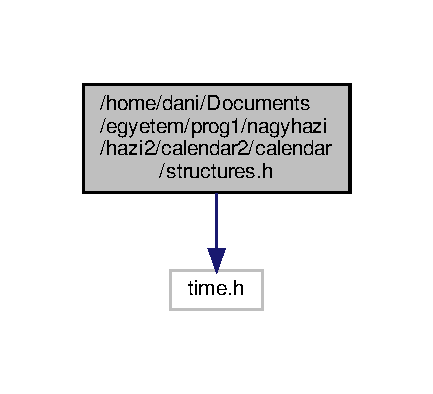
\includegraphics[width=208pt]{structures_8h__incl}
\end{center}
\end{figure}
This graph shows which files directly or indirectly include this file\+:\nopagebreak
\begin{figure}[H]
\begin{center}
\leavevmode
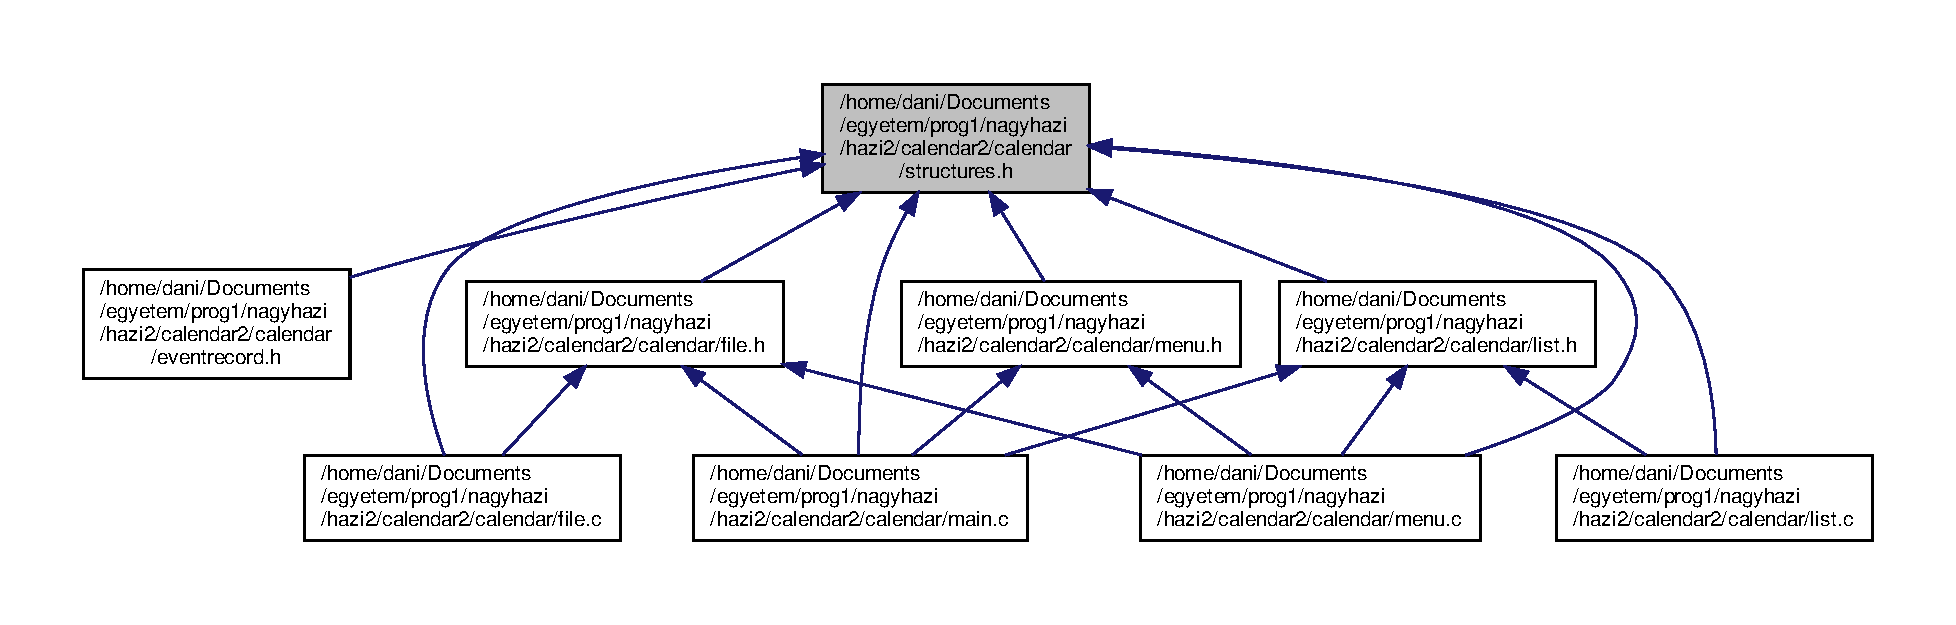
\includegraphics[width=350pt]{structures_8h__dep__incl}
\end{center}
\end{figure}
\subsection*{Data Structures}
\begin{DoxyCompactItemize}
\item 
struct \hyperlink{struct_event}{Event}
\item 
struct \hyperlink{struct_event_list}{Event\+List}
\item 
struct \hyperlink{struct_found_event}{Found\+Event}
\item 
struct \hyperlink{struct_find_list}{Find\+List}
\item 
struct \hyperlink{struct_search_conditions}{Search\+Conditions}
\item 
struct \hyperlink{struct_menu_pont}{Menu\+Pont}
\end{DoxyCompactItemize}
\subsection*{Typedefs}
\begin{DoxyCompactItemize}
\item 
typedef struct \hyperlink{struct_event}{Event} \hyperlink{structures_8h_a607b119a19e65e2c1c7a606f21ab7a46}{Event}
\item 
typedef struct \hyperlink{struct_event_list}{Event\+List} \hyperlink{structures_8h_a7faf24c32c52b92939a97982baf9dedf}{Event\+List}
\item 
typedef struct \hyperlink{struct_found_event}{Found\+Event} \hyperlink{structures_8h_ac0286403197d5147979a4986c9425222}{Found\+Event}
\item 
typedef struct \hyperlink{struct_find_list}{Find\+List} \hyperlink{structures_8h_ad7aca260cf976ef8a90cbe97ab5dba48}{Find\+List}
\item 
typedef struct \hyperlink{struct_search_conditions}{Search\+Conditions} \hyperlink{structures_8h_adc5706147428e7cb68faa6fb19085d7a}{Search\+Conditions}
\item 
typedef void($\ast$ \hyperlink{structures_8h_aa04041873905737ffeb12c611f7c5bde}{Menu\+Fv}) (\hyperlink{struct_event_list}{Event\+List} $\ast$)
\item 
typedef struct \hyperlink{struct_menu_pont}{Menu\+Pont} \hyperlink{structures_8h_a0ef80ab3e0ae7fe6915f17204e5f6211}{Menu\+Pont}
\item 
typedef struct tm \hyperlink{structures_8h_affc453d30a4a6ce81ed778fd04d2d256}{Tm}
\end{DoxyCompactItemize}


\subsection{Typedef Documentation}
\mbox{\Hypertarget{structures_8h_a607b119a19e65e2c1c7a606f21ab7a46}\label{structures_8h_a607b119a19e65e2c1c7a606f21ab7a46}} 
\index{structures.\+h@{structures.\+h}!Event@{Event}}
\index{Event@{Event}!structures.\+h@{structures.\+h}}
\subsubsection{\texorpdfstring{Event}{Event}}
{\footnotesize\ttfamily typedef struct \hyperlink{struct_event}{Event} \hyperlink{struct_event}{Event}}

\mbox{\Hypertarget{structures_8h_a7faf24c32c52b92939a97982baf9dedf}\label{structures_8h_a7faf24c32c52b92939a97982baf9dedf}} 
\index{structures.\+h@{structures.\+h}!Event\+List@{Event\+List}}
\index{Event\+List@{Event\+List}!structures.\+h@{structures.\+h}}
\subsubsection{\texorpdfstring{Event\+List}{EventList}}
{\footnotesize\ttfamily typedef struct \hyperlink{struct_event_list}{Event\+List} \hyperlink{struct_event_list}{Event\+List}}

\mbox{\Hypertarget{structures_8h_ad7aca260cf976ef8a90cbe97ab5dba48}\label{structures_8h_ad7aca260cf976ef8a90cbe97ab5dba48}} 
\index{structures.\+h@{structures.\+h}!Find\+List@{Find\+List}}
\index{Find\+List@{Find\+List}!structures.\+h@{structures.\+h}}
\subsubsection{\texorpdfstring{Find\+List}{FindList}}
{\footnotesize\ttfamily typedef struct \hyperlink{struct_find_list}{Find\+List} \hyperlink{struct_find_list}{Find\+List}}

\mbox{\Hypertarget{structures_8h_ac0286403197d5147979a4986c9425222}\label{structures_8h_ac0286403197d5147979a4986c9425222}} 
\index{structures.\+h@{structures.\+h}!Found\+Event@{Found\+Event}}
\index{Found\+Event@{Found\+Event}!structures.\+h@{structures.\+h}}
\subsubsection{\texorpdfstring{Found\+Event}{FoundEvent}}
{\footnotesize\ttfamily typedef struct \hyperlink{struct_found_event}{Found\+Event} \hyperlink{struct_found_event}{Found\+Event}}

\mbox{\Hypertarget{structures_8h_aa04041873905737ffeb12c611f7c5bde}\label{structures_8h_aa04041873905737ffeb12c611f7c5bde}} 
\index{structures.\+h@{structures.\+h}!Menu\+Fv@{Menu\+Fv}}
\index{Menu\+Fv@{Menu\+Fv}!structures.\+h@{structures.\+h}}
\subsubsection{\texorpdfstring{Menu\+Fv}{MenuFv}}
{\footnotesize\ttfamily typedef void($\ast$ Menu\+Fv) (\hyperlink{struct_event_list}{Event\+List} $\ast$)}

\mbox{\Hypertarget{structures_8h_a0ef80ab3e0ae7fe6915f17204e5f6211}\label{structures_8h_a0ef80ab3e0ae7fe6915f17204e5f6211}} 
\index{structures.\+h@{structures.\+h}!Menu\+Pont@{Menu\+Pont}}
\index{Menu\+Pont@{Menu\+Pont}!structures.\+h@{structures.\+h}}
\subsubsection{\texorpdfstring{Menu\+Pont}{MenuPont}}
{\footnotesize\ttfamily typedef struct \hyperlink{struct_menu_pont}{Menu\+Pont}  \hyperlink{struct_menu_pont}{Menu\+Pont}}

\mbox{\Hypertarget{structures_8h_adc5706147428e7cb68faa6fb19085d7a}\label{structures_8h_adc5706147428e7cb68faa6fb19085d7a}} 
\index{structures.\+h@{structures.\+h}!Search\+Conditions@{Search\+Conditions}}
\index{Search\+Conditions@{Search\+Conditions}!structures.\+h@{structures.\+h}}
\subsubsection{\texorpdfstring{Search\+Conditions}{SearchConditions}}
{\footnotesize\ttfamily typedef struct \hyperlink{struct_search_conditions}{Search\+Conditions} \hyperlink{struct_search_conditions}{Search\+Conditions}}

\mbox{\Hypertarget{structures_8h_affc453d30a4a6ce81ed778fd04d2d256}\label{structures_8h_affc453d30a4a6ce81ed778fd04d2d256}} 
\index{structures.\+h@{structures.\+h}!Tm@{Tm}}
\index{Tm@{Tm}!structures.\+h@{structures.\+h}}
\subsubsection{\texorpdfstring{Tm}{Tm}}
{\footnotesize\ttfamily typedef struct tm \hyperlink{list_8h_affc453d30a4a6ce81ed778fd04d2d256}{Tm}}


%--- End generated contents ---

% Index
\backmatter
\newpage
\phantomsection
\clearemptydoublepage
\addcontentsline{toc}{chapter}{Index}
\printindex

\end{document}
